\documentclass[
  a4paper,
  abstract=true,
  twoside,
  listof=totoc,
  numbers=noenddot,
  bibliography=totoc,
  BCOR1.5cm,
  headsepline,
  DIV12,
  appendixprefix,
  final
] {scrreprt}

% You should select either american or british instead of english here:
\usepackage[ngerman]{babel}
\usepackage{lmodern}
%\usepackage{fontspec}
\usepackage{afterpage}
\usepackage{tabularx}
\usepackage{mwe}
\usepackage{booktabs}
\usepackage{adjustbox}
\usepackage{subcaption}
\usepackage[pdftex,
citebordercolor={0.75 0.75 1},
filebordercolor={0.75 0.75 1},
linkbordercolor={0.75 0.75 1},
pagebordercolor={0.75 0.75 1},
urlbordercolor={0.75 0.75 1},
pdfborder={0.75 0.75 1},plainpages=false,pdfpagelabels=true]{hyperref}
\hypersetup{
  pdftitle={Low Latency-Kryptographie für transparente Layer 2 - Verschlüsselung mit MACsec},
  pdfauthor={Gregor Garten},
  pdfkeywords={foo, bar},
}
\usepackage[acronym,nomain,toc]{glossaries}



\usepackage[backend=biber,style=alphabetic,alldates=long]{biblatex}

\usepackage{varioref}           % nice refs
\usepackage{csquotes}
\usepackage{graphicx}           % graphics
\usepackage{caption}            % manipulate fugures
\usepackage{subcaption}         % allow for subfigures
\usepackage{listings}           % nice source code listings
\usepackage{color}
\usepackage{booktabs}           % nice tables
\usepackage{microtype}          % better looking text borders
\usepackage{units}              % unified way of setting values with units
\usepackage{array}
\usepackage{fancybox}           % provide nice boxes
\usepackage{units}              % unified way of setting values with units
\usepackage{fancyvrb}           % algorithm-boxes
\usepackage{pdfpages}
\usepackage{hyphenat}
\usepackage{todonotes}
\usepackage{xspace}
\usepackage{setspace}

% use this one last
% (redefines some macros for compatibility with KOMAScript)
\usepackage{scrhack}

\addbibresource{Literaturverzeichnis.bib}
 
\definecolor{mygreen}{rgb}{0,0.6,0}
\definecolor{mygray}{rgb}{0.5,0.5,0.5}
\definecolor{mymauve}{rgb}{0.58,0,0.82}
 
% Biblatex Style
\setcounter{secnumdepth}{3}     % limit enumeration depth
\setcounter{tocdepth}{1}        % limit TOC depth

% Listing Style

\lstset{ %
  frame=shadowbox,
  rulesepcolor=\color{blue},
  backgroundcolor=\color{white},   % choose the background color; you must add \usepackage{color} or \usepackage{xcolor}
%  basicstyle=\footnotesize,        % the size of the fonts that are used for the code
  breakatwhitespace=false,         % sets if automatic breaks should only happen at whitespace
  breaklines=true,                 % sets automatic line breaking
  captionpos=b,                    % sets the caption-position to bottom
  commentstyle=\color{mygreen},    % comment style
  deletekeywords={...},            % if you want to delete keywords from the given language
  escapeinside={\%*}{*)},          % if you want to add LaTeX within your code
  extendedchars=true,              % lets you use non-ASCII characters; for 8-bits encodings only, does not work with UTF-8
  frame=single,                    % adds a frame around the code
  keepspaces=true,                 % keeps spaces in text, useful for keeping indentation of code (possibly needs columns=flexible)
  keywordstyle=\color{blue},       % keyword style
  language=C,                 % the language of the code
 % morekeywords={*,...},            % if you want to add more keywords to the set
  numbers=left,                    % where to put the line-numbers; possible values are (none, left, right)
  numbersep=7pt,                   % how far the line-numbers are from the code
  numberstyle=\tiny\color{mygray}, % the style that is used for the line-numbers
  rulecolor=\color{black},         % if not set, the frame-color may be changed on line-breaks within not-black text (e.g. comments (green here))
  showspaces=false,                % show spaces everywhere adding particular underscores; it overrides 'showstringspaces'
  showstringspaces=false,          % underline spaces within strings only
  showtabs=false,                  % show tabs within strings adding particular underscores
  stepnumber=1,                    % the step between two line-numbers. If it's 1, each line will be numbered
  stringstyle=\color{mymauve},     % string literal style
  tabsize=2,                       % sets default tabsize to 2 spaces
  title=\lstname                   % show the filename of files included with \lstinputlisting; also try caption instead of title
}

% Typesetting options
\tolerance 2414
\hbadness 2414
\emergencystretch 1.5em
\hfuzz 0.3pt
\widowpenalty=10000     % Hurenkinder
\clubpenalty=10000      % Schusterjungen
\vfuzz \hfuzz
\raggedbottom

% use nice footnote indentation
\deffootnote[1em]{1em}{1em}{\textsuperscript{\thefootnotemark}\,}
 
% some common commands
\newcommand{\drops}{\texorpdfstring{\textsc{Drops}\xspace}{DROPS}}
\newcommand{\LLinux}{\texorpdfstring{L$\!^4$Linux}{L4Linux}}

\newcommand{\NOVA}{NOVA\xspace}
\newcommand{\QEMU}{QEMU\xspace}
\glsdisablehyper
\setacronymstyle{long-em-short}


\newacronym{IEEE}{IEEE}{Institute of Electrical and Electronics Engineers}
\newacronym{ISO}{ISO}{International Standards Organization}
\newacronym{MACsec}{MACsec}{Medium Access Control Security}
\newacronym{OSI-Modell}{OSI-Modell}{Open Systems Interconnection Model}
\newacronym{AEAD}{AEAD}{Authenticated Encryption with Associated Data}
\newacronym{AES}{AES}{Advanced Encryption Standard}
\newacronym[plural=AES-GCM,firstplural=Galois Counter Mode (AES-GCM)]{AES-GCM}{AES-GCM}{Advanced Encryption Standard with Galois Counter Mode}
\newacronym{AES-NI}{AES-NI}{Advanced Encryption Standard New Instructions}
\newacronym{CAESAR}{CAESAR}{Competition for Authenticated Encryption: Security, Applicability, and Robustness}
\newacronym{MAC}{MAC}{Medium Access Control}
\newacronym{LLC}{LLC}{Logical Link Control}
\newacronym{ICMP}{ICMP}{Internet Control Message Protocol}
\newacronym{TCP}{TCP}{Transmission Control Protocol}
%\newacronym{MAC}{MAC}{Message Authentikation Codes}
\newacronym{K}{K}{symmetrischen Schlüssel}
\newacronym{IV}{IV}{Initialisierungsvektor}
\newacronym{M}{M}{Klartext}
\newacronym{C}{C}{Chiffrat}
\newacronym{AD}{AD}{associated Data}
\newacronym{DoS}{DoS}{Denial of Service}
\newacronym{M}{M}{Klartext}
\newacronym{SecY}{SecY}{MAC Security Entity}
\newacronym{KaY}{KaY}{Security Key Agreement Entity}
\newacronym{MKA}{MKA}{MACsec Key Agreement Protokoll}
\newacronym{CA}{CA}{Connectivity Association}
\newacronym[plural=SC,firstplural=Secure Channels (SC)]{SC}{SC}{Secure Channel}
\newacronym[plural=SA,firstplural=Secure Associations (SA)]{SA}{SA}{Secure Association}
\newacronym{SAK}{SAK}{Secure Association Key }
\newacronym{SCI}{SCI}{Secure Channel Identifier}
\newacronym{ICV}{ICV}{Integrity Check Value}
\newacronym{AN}{AN}{Association Number}
\newacronym{TCI}{TCI}{TAG Control Information Feld}
\newacronym{PPP}{PPP}{Point-to-Point Protocol}
\newacronym{NIST}{NIST}{National Institute of Standards and Technology}
\newacronym{ES}{ES}{End Station Bit}
\newacronym{SSE}{SSE}{Streaming Simd Extensions}
\newacronym{AVX}{AVX}{Advanced Vector Extensions Befehlssatzerweiterung}
\newacronym{DES}{DES}{Data Encryption Standard}
\newacronym[plural=CPU,firstplural=Central Processing Units (CPU)]{CPU}{CPU}{Central Processing Unit}
\newacronym{SUPERCOP}{SUPERCOP}{System for Unified Performance Evaluation related to Cryptographic Operations and Primitives}
\newacronym{API}{API}{Application Programming Interface}
\newacronym{SoC}{SoC}{System on Chip }
\newacronym{SSH}{SSH}{Secure Shell}
\newacronym{DES}{DES}{Data Encryption Standard}
\newacronym{DES}{DES}{Data Encryption Standard}
\newacronym{DES}{DES}{Data Encryption Standard}
\newacronym{DES}{DES}{Data Encryption Standard}




\makeglossaries
%\makeglossary
% If you know when you will hand in your thesis, enter the date here.
%\date{30. April 2009}
%\newcommand{\printdate}{\@date}

\begin{document}


\pagenumbering{Roman}

 
\selectlanguage{ngerman}

\begin{singlespace}

\subject{{\LARGE Bachelorarbeit}}

\title{Low Latency-Kryptographie für transparente Layer 2 - Verschlüsselung mit MACsec}

\author{Gregor Garten}

\publishers{Technische Universität Dresden\\
Fakultät Informatik\\
Institut für Systemarchitektur\\
Professur Datenschutz und Datensicherheit\\
\begin{minipage}{\textwidth}%\\
\vskip 6cm
 {\normalsize }\begin{tabular}{ll}
Betreuender Hochschullehrer: &
Prof. Dr. rer. nat. Thorsten Strufe\tabularnewline
Betreuende Mitarbeiter: &
Dr.-Ing. Stefan Köpsell \tabularnewline 
& Dipl.-Inf.  Tim Lackorzynski  \tabularnewline
\end{tabular} {\normalsize }\end{minipage}}

\maketitle
\end{singlespace}

\cleardoublepage

%
\includepdf{images/diplom-aufgabe.pdf}
\cleardoublepage
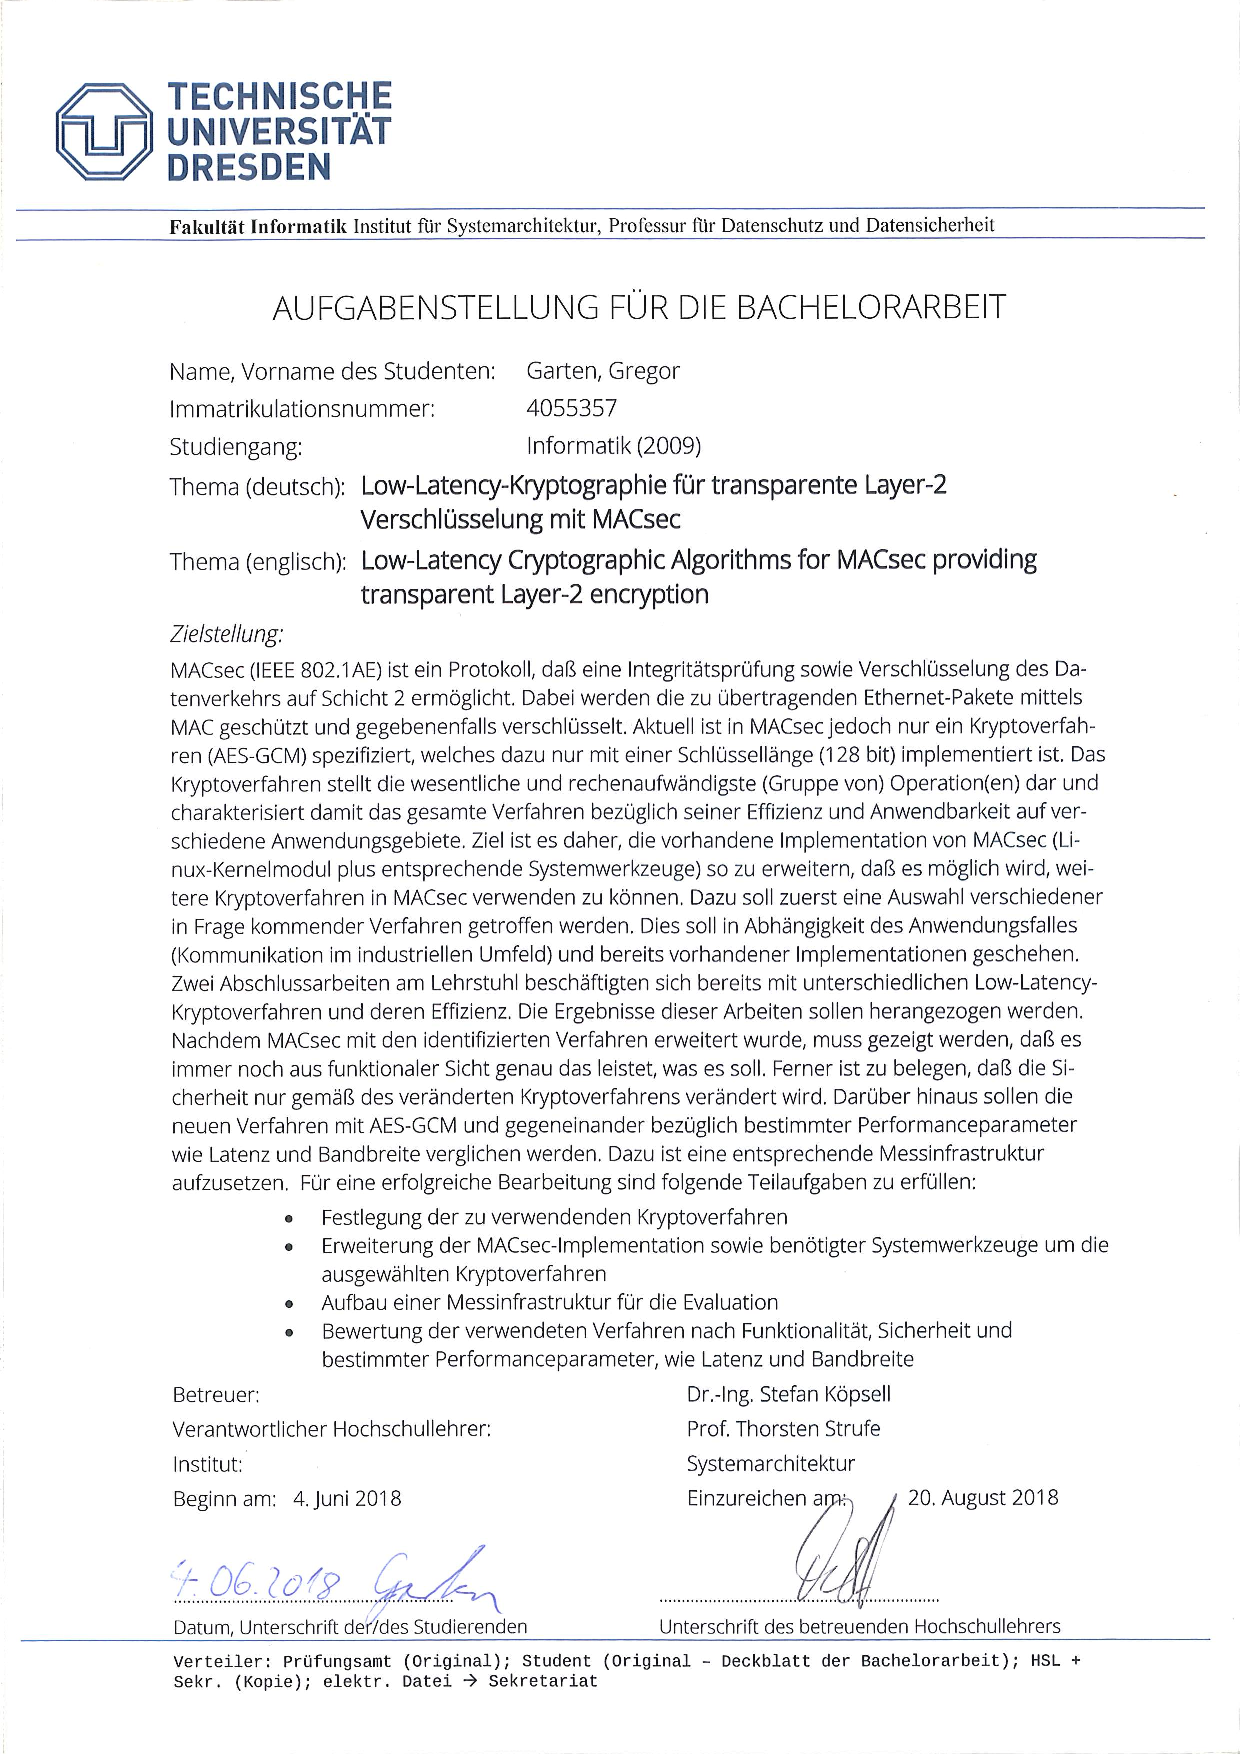
\includepdf{./Aufgabenstellung.pdf}

 
\selectlanguage{ngerman}

\section*{\vfill{} \thispagestyle{empty}
Erklärung}

Hiermit erkläre ich, dass ich diese Arbeit selbstständig erstellt
und keine anderen als die angegebenen Hilfsmittel benutzt habe.
\bigskip{}

\noindent Dresden, den \today % \printdate % if you defined date earlier
\vspace{2.5cm}

\noindent Gregor Garten \cleardoublepage{}

% NOTE: if you selected british or american above, change that here too
\selectlanguage{ngerman}

%\begin{abstract}
%% -*- Mode: Latex -*-

%  Zusammenfassung

% Zu einer runden Arbeit gehört auch eine Zusammenfassung, die
% eigenständig einen kurzen Abriß der Arbeit gibt. Eine halbe bis ganze
% DINA4 Seite ist angemessen. Dafür läßt sich keine Gebrauchsanweisung
% geben (für irgendetwas müssen die Betreuer ja auch noch da
% sein).

\ldots abstract \ldots


%%% Local Variables:
%%% TeX-master: "diplom"
%%% End:



%\end{abstract}

\tableofcontents

% remove this on final

\listoffigures

\listoftables
\cleardoublepage

\pagenumbering{arabic}
\chapter{Einleitung}
\label{sec:intro}

% Die Einleitung schreibt man zuletzt, wenn die Arbeit im Großen und
% Ganzen schon fertig ist. (Wenn man mit der Einleitung beginnt - ein
% häufiger Fehler - braucht man viel länger und wirft sie später doch
% wieder weg). Sie hat als wesentliche Aufgabe, den Kontext für die
% unterschiedlichen Klassen von Lesern herzustellen. Man muß hier die
% Leser für sich gewinnen. Das Problem, mit dem sich die Arbeit befaßt,
% sollte am Ende wenigstens in Grundzügen klar sein und dem Leser
% interessant erscheinen. Das Kapitel schließt mit einer Übersicht über
% den Rest der Arbeit ab. Meist braucht man mindestens 4 Seiten dafür, mehr
% als 10 Seiten liest keiner.
Die Digitalisierung zählt zu den großen Herausforderungen der gegenwärtigen Zeit und auch für die Zukunft. Es erfordert umfangreiche Anpassungen unter anderem in der Industrie.
In der Bachelorarbeit sollen für diese zentrale Aufgabe zunächst einige Grundlagen dargestellt, um dann Lösungswege zur Verbesserung untersucht und herausgearbeitet werden.\\
Es ist neben der Vernetzung von Systemen eines der Hauptziele der Industrie 4.0, die entstehenden Datenaufkommen zu sichern. Jedoch entstehen mit der zunehmenden Vernetzung von Komponenten innerhalb eines Unternehmens neue Möglichkeiten, um in ein Netzwerk einzudringen und Daten unerlaubt abzuschöpfen. Das fastvpn Projekt hat hierfür ein Sicherheitskonzept entwickelt, das sich diesem Problem widmet \cite{fastvpn2018}.
Hierfür kommunizieren sicherheitsrelevante Systeme mit FastVPN-Boxen, die eine sichere Kommunikationsübertragung bereitstellen können und als Vermittler zwischen den sicherheitsrelevanten Systemen fungieren. 
Mit der Anforderung der Echtzeitkommunikation in der Industrie 4.0 werden enorme Ansprüche an Netzwerksicherheitsstandards gesetzt. Diese müssen nicht nur die größtmöglichste Sicherheit gewährleisten, sondern auch geringe Auswirkungen auf die Übertragungszeit von Nachrichten haben. Daher wird die Performance von Netzwerkprotokollen zu einem entscheidenden Kriterium. 
\\
Eines der Netzwerkprotokolle, welches für die Sicherheit in den FastVPN-Boxen zuständig ist, ist der \gls{IEEE} Sicherheitsstandard \gls{MACsec}. \gls{MACsec} arbeitet auf der zweiten Schicht des \gls{OSI-Modell} und nutzt den  Betriebsmodus \gls{AEAD}. Dadurch können gleich mehrere Sicherheitsziele, darunter Vertraulichkeit und Integrität durch nur einen Verschlüsselungsalgorithmus erreicht werden. Der verwendete Verschlüsselungsalgorithmus ist der \gls{AES}, der im  \glspl{AES-GCM} betrieben wird. \gls{AES} ist einer der meistgenutzten Verschlüsselungsalgorithmen, der in diversen Sicherheitsprotokollen benutzt wird. Durch die weite Verbreitung von \gls{AES} findet sich in fast jedem Computer die Hardware Unterstützung \gls{AES-NI} wieder, von der der Algorithmus zusätzlich profitiert. Die Verbreitung von \gls{AES} bringt allerdings auch diverse Probleme mit sich. \gls{AES-GCM} nutzt eine der rechenaufwändigsten Operationen und kann ohne Hardware Unterstützung nicht mit anderen neueren Verschlüsselungsalgorithmen mithalten.\\  
Mit Blick auf den Anwendungsfall der industriellen Kommunikation ist es daher sinnvoll, nach anderen Verschlüsselungsalgorithmen zu suchen, die möglicherweise eine bessere Performance erreichen können, da die Systeme im industriellen Bereich oft keine \gls{AES-NI} Hardware Unterstützung beherbergen. Um eine effiziente Alternative zu besitzen, sollte der Verschlüsselungsalgorithmus nicht von der Hardware Unterstützung abhängig sein, um eine gute Performance zu erreichen. 
Diese Arbeit widmet sich dem Problemfall und setzt sich das Ziel nach einem vielversprechenden Verschlüsselungsalgorithmus zu suchen, der eine Alternative zu \gls{AES-GCM} bieten kann. \\
Dafür muss eine Auswahl aus potentiellen Verschlüsselungsalgorithmen getroffen werden, die daraufhin in das \gls{MACsec} Modul implementiert werden. Des Weiteren muss überprüft werden, ob sich durch einen Austausch der Verschlüsselungskomponente eine Performancesteigerung des Sicherheitsstandards erreichen lässt. Dafür wird eine Testumgebung kreiert und Performance Tests durchgeführt.
Um einen Einblick in die Thematik zu geben, werden im nächsten Kapitel die Grundlagen erklärt. Daraufhin werden Verschlüsselungsalgorithmen vorgestellt, die mögliche Kandidaten für eine Erweiterung in das MACsec Modul sind. Danach werden die Änderungen beschrieben, die im MACsec Modul getätigt werden müssen, um zusätzliche Verschlüsselungsalgorithmen nutzen zu können. Diese werden nach den Kriterien der Sicherheit, Funktionalität und Geschwindigkeit bewertet. Zum Schluss wird ein Fazit aus den Ergebnissen der Analyse gezogen.




%\section{Forschungsstand} 
%%\\
%\\
%Bisher wurde die MACsec Implementierung mit keinen weiteren %Verschlüsselungsalgorithmen erweitert.
%Aber es existiert bereits ein \gls{IEEE} Standard, indem %MACsec um einen Algorithmus erweitert wird \cite{6047536}. Die Erfahrung zeit jedoch, dass eine Erweiterung der  Implementation viel Zeit in Anspruch nimmt, da allein schon der  Integration eines zusätzlichen Verschlüsselungsalgorithmus benötigt viel Zeit und derzeit gibt es noch keine Pläne diesen Standard in das Linux Betriebssystem zu integrieren. Allein

%Zeitgleich läuft ein kryptografischer Wettbewerb namens \gls{CAESAR}, der nach Chiffren mit Vorteilen gegenüber \gls{AES-GCM} sucht. Auf die Resultate des Wettbewerbs wird ebenfalls eingegangen.
% meistverbreiteste Verschlüsselungsalgorithmus. AES ist in fast jedem Netzwerkfähigen Gerät aufzufinden und das nicht ohne Grund. AES überzeugt mit einem gutem Design, von Hardware Unterstützungen wie AES-NI und einer hohen Performance. Deshalb wird AES in einer Vielzahl von Netzwerkprotokollen verwendet unter anderem auch im Sicherheitsstandard MACsec. MACsec ist ein Netzwerksicherungsprotokoll
%Something with umlauts and a year/month date:
%\cite{becher04:_feurig_hacken_mit_firew}.

%And some online resources: \cite{green04}, \cite{patent:4819234}



%%% Local Variables:
%%% TeX-master: "diplom"
%%% End:

\chapter{Grundlagen}
\label{sec:state}

% Hier werden zwei wesentliche Aufgaben erledigt:

% 1. Der Leser muß alles beigebracht bekommen, was er zum Verständnis
% der späteren Kapitel braucht. Insbesondere sind in unserem Fach die
% Systemvoraussetzungen zu klären, die man später benutzt. Zulässig ist
% auch, daß man hier auf Tutorials oder Ähnliches verweist, die hier auf
% dem Netz zugänglich sind.
% 2. Es muß klar werden, was anderswo zu diesem Problem gearbeitet
% wird. Insbesondere sollen natürlich die Lücken der anderen klar
% werden. Warum ist die eigene Arbeit, der eigene Ansatz wichtig, um
% hier den Stand der Technik weiterzubringen? Dieses Kapitel wird von
% vielen Lesern übergangen (nicht aber vom Gutachter ;-), auch später
% bei Veröffentlichungen ist "Related Work" eine wichtige Sache.

% Viele Leser stellen dann später fest, daß sie einige der Grundlagen
% doch brauchen und blättern zurück. Deshalb ist es gut,
% Rückwärtsverweise in späteren Kapiteln zu haben, und zwar so, daß man
% die Abschnitte, auf die verwiesen wird, auch für sich lesen
% kann. Diese Kapitel kann relativ lang werden, je größer der Kontext
% der Arbeit, desto länger. Es lohnt sich auch! Den Text kann man unter
% Umständen wiederverwenden, indem man ihn als "Tutorial" zu einem
% Gebiet auch dem Netz zugänglich macht.

% Dadurch gewinnt man manchmal wertvolle Hinweise von Kollegen. Dieses
% Kapitel wird in der Regel zuerst geschrieben und ist das Einfachste
Um einen Überblick in die Grundlagen dieser Bachelorarbeit zu geben, erfolgt in diesem Kapitel zunächst die Erläuterung zentraler Begriffe der Netzwerktheorie. Das ist eine wichtige Voraussetzung, um die Funktionsweise vom Sicherheitsstandard \gls{MACsec} verstehen zu können. Danach werden grundlegende im Standard benutzte Sicherheitsbegriffe beschrieben, um anschließend auf den Standard als solches, dessen Funktion und Sicherheitsziele einzugehen. Falls es nicht anders erwähnt wird, werden die Kenntnisse für den Abschnitt 2.1 aus \cite{TN_libero_mab23259530} entnommen.
\section{Netzwerktheorie}
% (oder das Schwerste weil erste).
%In diesem Kapitel werden als erstes zentrale Begriffe der Netzwerktheorie erklärt, die essentiell sind, um die Funktionsweise vom Sicherheitsstandard MACsec zu verstehen. Danach werden grundlegende Sicherheitsbegriffe und Verfahren darstellen, die im Standard benutzt werden. Anschließend erfolgt die Beschreibung des MACsec Standards,( wie es funktioniert, was geschützt wird und welche Sicherheitsziele verfolgt werden.)
%zentrale Begriffe der Netzwerktheorie und der Kryptographie, die zum Verständnis der Bachelorarbeit essentiell sind, eingeführt und erläutert.
%Um das Verständnis 


\textbf{OSI Referenzmodell} \\
\\
Das OSI Referenzmodell wurde von der \gls{ISO} entwickelt. Es war der erste Versuch  Kommunikationsprotokolle zu standardisieren, um zwischen verschiedenen technischen Systemen zu kommunizieren. Das \gls{OSI-Modell} besteht aus sieben Schichten, wobei jede einzelne Schicht eine genau definierte Funktion erfüllt. Wenn eine Nachricht von einem zum anderen Computer geschickt wird, durchläuft die Nachricht zuerst alle 7 Schichten auf dem Computer des Senders und ein zweites Mal alle 7 Schichten auf dem Computer des Empfängers. Für den Gegenstand der Bachelorarbeit ist die Sicherungsschicht von besonderer Bedeutung, da \gls{MACsec} selbst auf der 2. Schicht des \gls{OSI-Modell}s arbeitet und Kenntnisse aus dieser Schicht relevant zum Verständnis dieser Arbeit sind.\\
\\
\textbf{Sicherungsschicht}\\ 
\\
Die Sicherungsschicht ist die zweite Ebene des \gls{OSI-Modell}s. Ihre Aufgabe ist es den Bitstrom aus der Bitübertragungsschicht (Schicht 1) in Blöcke, die Rahmen genannt werden, aufzuteilen und an die Vermittlungsschicht (Schicht 3) weiterzuleiten. So muss durch die Sicherungsschicht eine zuverlässige Übertragung der Daten gewährleistet werden. Hierfür werden zusätzliche Redundanzen zum Rahmen hinzugefügt, um gesendete Informationen auf Fehler zu prüfen und Maßnahmen der Fehlerkorrektur durchführen zu können. Deshalb muss in der Vermittlungsschicht nicht mehr auf grobe Fehler in dem Datenpaket geprüft werden. Ein weiteres wichtiges Kriterium ist die Regulierung des Datenflusses durch den Empfänger. Dies dient dazu, dass es nicht zu einer Überlastung des Empfängers kommt, falls der Sender schneller Daten sendet als der Empfänger annehmen kann. Die Sicherungsschicht wird in zwei Teilschichten untergliedert, die \gls{MAC} und die \gls{LLC}. \\
\\\\
\textbf{Medium Access Control}\\\\
In der Medium Access Control Teilschicht werden die vorhandenen Kommunikationskanäle zwischen den Mitgliedern innerhalb eines Netzwerks organisiert. Hierbei wird während der Übertragung überprüft, ob es zu einer Kollision auf dem Kanal zwischen den Kommunikationspartnern gekommen ist. Im Falle einer Kollision werden je nach Protokoll unterschiedliche Maßnahmen ergriffen, um die Kollisionsgefahr auf dem Kanal zu verringern. Allerdings müssen bei einer Kollision die Nachrichten generell erneut gesendet werden. In der Literatur findet man auch kollisionsfreie Übertragungsprotokolle, diese finden in der Praxis jedoch kaum Anwendung. 
%In der Medium Access Controll Teilschicht werden Verfahren zur Kollisionsbereinigung 
%broadcast kanal wird mehreren benutzern bereitgestellt, Von %einer Kollision ist die Rede, wenn beide Kommunikationsstationen eine Nachricht zum gleichen Zeitpunkt senden. einer Nachricht auf dem Kanal gemeint. führt zu kollisionen.\\
\\
\\
\textbf{Ethernet}
\\
\\
Ethernet wurde unter dem Begriff \gls{IEEE} Norm 802.3 standardisiert. Daher können \gls{IEEE} Norm 802.3 und Ethernet als Synonym verwendet werden. In dieser Bachelorarbeit wird stets der Begriff Ethernet verwendet, da dies die gängigste Verbreitung des Ausdrucks ist. Ethernet beschreibt im Allgemeinen die physische Verbindung von 2 Systemen mittels eines Kabels, wodurch die Kommunikation der beiden Systeme erfolgt.\\
\\
\begin{figure}
	\centering
	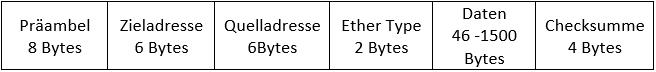
\includegraphics[width=0.9\textwidth]{images/Ethernet_Rahmen.PNG}
	\caption[Felder eines Ethernet Rahmen]{In der Abbildung werden die 6 Bestandteile eines Ethernet Rahmen gezeigt. Dazu wird die Größe eines Feldes in Bytes angezeigt. }
	\label{img:Rahmen}
\end{figure}\textbf{Ethernet auf der MAC-Teilschicht}\\
\\\label{sec: Ethernet auf der MAC-Teilschicht}
Die Daten, die über die \gls{MAC}-Teilschicht des \gls{OSI-Modell}s laufen, werden in der Fachliteratur als Rahmen bezeichnet. Deshalb wird im Verlauf der Arbeit stets der Begriff Rahmen für diese Daten übernommen. Ein Rahmen beim Ethernet in der \gls{MAC}-Teilschicht weist folgende Struktur auf. Als erstes beginnt ein Rahmen mit einer Präambel, die eine Länge von 8 Bytes aufweist, wobei jedes Byte das Bitmuster 10101010 besitzt, ausgenommen sind die letzten beiden Bits. Diese werden auf 11 gesetzt. Dies hat den Zweck, Empfänger und Sender zu synchronisieren. Als nächstes folgen zwei 6 Bytes lange Stücke. Der erste Teil beinhaltet die \gls{MAC}-Addresse des Empfängers und der zweite die des Senders. Eine Besonderheit der \gls{MAC}-Adresse ist dadurch gekennzeichnet, dass die Vergabe nur von der \gls{IEEE} erfolgt und jede \gls{MAC}-Adresse global einzigartig ist. Anschließend wird die Länge des Rahmens in einem 2 Byte großem Feld angegeben. In neueren Ethernet Versionen wird das 2 Byte große Feld zum Typ Feld, sodass Protokolle mittels des Typ Feldes unterschieden werden können. Danach folgt nun das Daten Feld, in denen sich die zu sendenden Daten befinden. Das Daten Feld ist maximal 1500 Bytes groß. Also kann ein Rahmen in der \gls{MAC}-Teilschicht eine maximale Größe von 1518 Bytes haben, wenn man die Größe des Headers und Trailers hinzurechnet. Außerdem gibt es auch eine Mindestgröße des Daten Feldes von 46 Bytes. Sollte eine Nachricht trotzdem kleiner sein, so wird die Nachricht mit Nullen auf 46 Bytes aufgefüllt. Daraus folgt, dass ein kompletter Rahmen mindestens eine Größe von 64 Bytes hat. Dies ist die minimale Größe, die benötigt wird, um die Verfahren zur Kollisionserkennung gewährleisten zu können. Ansonsten ist die ganze Nachricht bereits gesendet, bevor der Empfänger realisieren kann, dass eine Kollision vorlag. Zuletzt kommt ein 4 Byte großes Feld, in dem sich die Checksumme befindet. Durch die Checksumme kann überprüft werden, ob die Nachricht korrekt übertragen wurde. Falls dies nicht der Fall sein sollte, kann der Empfänger ein Signal senden, damit der Sender den Rahmen erneut überträgt. Nach einer übermittelten Nachricht wird eine 9,6 \textmu s lange Sendepause eingelegt.
Die Struktur eines Ethernet Rahmens mit seinen einzelnen Feldern ist in der Abbildung \ref{img:Rahmen} zu sehen. \\
\\
\textbf{ICMP}\\
\\
Das \gls{ICMP} ist ein Steuerprotokoll, welches auf der Vermittlungsschicht arbeitet. Sollte im Verlauf einer Paketübertragung ein Router ausfallen oder ein anderes Problem auftreten, so wird dem Sender durch das \gls{ICMP} ein Paket übermittelt, in dem der Sender über das Ereignis informiert wird. 
%An dieser Stelle sollte hervorgehoben werden, dass nur einige Fehlermeldungen erkannt werden 
Eine Liste der unterstützten Nachrichten findet man unter \cite{ICMP}.\\
\\
\textbf{TCP}
\\
\\
Das \gls{TCP} ist ein Internetübertragungsprotokoll, das eine zuverlässige Übertragung garantiert. Außerdem wird bei \gls{TCP} auf die Reihenfolge der Pakete wert gelegt. Es wird in der der Transportschicht des \gls{OSI-Modell}s, der 4. Schicht, eingesetzt. Auch wenn die vorhandenen Netzwerke unzuverlässig sind, kann sich das \gls{TCP} robust auf alle Arten von Fehlern einstellen. Beim \gls{TCP}-Protokoll werden übertragende Daten als Segmente bezeichnet. Ein \gls{TCP}-Segment fängt mit einem 20-Byte langem Header an, gefolgt von einem optionalen Teil und anschließend von einem Datenbytes-Feld, das auch, anders als bei Ethernet, keine Daten enthalten kann.
\section{Sicherheit}\\
\\
In diesem Abschnitt werden einige Grundlagen der Sicherheit in Rechnernetzen erläutert, die für das Verständnis der Funktionsweise des Sicherheitsstandards MACsec von Bedeutung sind. Die Informationen für diesen Abschnitt sind aus \cite{pfitzmann2000sicherheit} entnommen.
\\
\\
\textbf{Sicherheitsziele}\\
\\
Es wird im Allgemeinen in 3 Sicherheitsziele unterteilt:
\begin{itemize}
\item Vertraulichkeit: Es ist nicht möglich, dass eine unautorisierte Partei einen Informationsgewinn über den Inhalt der gesendeten Daten erhält.
\item Integrität: Es ist nicht möglich, dass eine unautorisierte Partei den Inhalt von Daten modifizieren kann, ohne das dies bemerkt wird.
\item Verfügbarkeit: Es ist nicht möglich, dass eine unautorisierte Partei die Funktionalität eines Dienstes beeinträchtigen kann.
\end{itemize} \\
In dieser Arbeit ist noch ein 4. Sicherheitsziel von Bedeutung:
\begin{itemize}
\item Authentizität: Eine gesendete Nachricht kann einem Sender zugeordnet werden.\\
\end{itemize}
\\
\textbf{Symmetrisches Konzelationssystem}\\
\\
Bei einem symmetrischen Konzelationssystem wird ein zufälliger Schlüssel generiert, der zwischen Sender und Empfänger ausgetauscht wird. Dieser Schlüssel wird sowohl bei der Verschlüsselung als auch Entschlüsselung von Nachrichten angewendet. Mit einem symmetrischen Konzelationssystem kann das Schutzziel der Vertraulichkeit erfüllt werden. \\
\\
\textbf{Symmetrisches Authentikationssystem}\\
\\
%Authentikations oder Authentifikationssytem?
Bei einem symmetrischen Authentikationssystem wird ebenfalls ein zufälliger Schlüssel generiert, der zwischen Sender und Empfänger ausgetauscht wird. Anders als bei einem Konzelationssystem werden die ausgetauschten Nachrichten nicht verschlüsselt und entschlüsselt, sondern es wird ein Prüfteil an die zu sendende Nachricht angefügt. Der Empfänger einer Nachricht kann mit dem richtigen Schlüssel den Prüfteil selbständig berechnen und vergleichen. Sollte sich der berechnete Prüfteil von der erhaltenen Nachricht unterscheiden, dann wurde die Nachricht verändert. Mit einem Authentikationssystem kann das Schutzziel der Integrität erfüllt werden. In der restlichen Arbeit wird der gängigere englische Begriff des Message Authentikation Codes \gls{MAC} anstelle des Authentikationssystems verwendet.\\
\\
\textbf{Replay-Angriff}\\
\\ 
Bei einem Replay-Angriff werden bereits gesendete Nachrichten von einem Angreifer gesammelt und erneut in den Nachrichtenfluss gestreut, meistens mit der Intention das Sicherheitsziel der Authentizität zu schwächen. \\  
\\
\textbf{bounded receive delay}\\
\\
Unter bounded receive delay versteht man, dass ein Man-in-the-Middle Angreifer keine Pakete in einem Netzwerk verzögern oder abfangen kann, ohne das dies von den Beteiligten in einem Netzwerk erkannt wird.
\\
\\
\\
\\
\textbf{Denial of Service}\\
\\
\gls{DoS} ist ein Angriff mit der Absicht, das Sicherheitsziel der Verfügbarkeit zu schwächen. Dazu werden an einen Server eine Vielzahl von Anfragen geschickt, bis der Server überlastet ist und diese nicht mehr beantworten kann. Der Server kann zu diesem Zeitpunkt keine sinnvollen Anfragen von Nutzern mehr beantworten, die auf den Service des Servers zugreifen wollen. Somit ist der Service für die Nutzer nicht mehr verfügbar.
\section{Authenticated Encryption with Associated Data}
\label{sec:Authenticated Encryption with Associated Data}
\\
\\
Authenticated Encryption with Associated Data (\gls{AEAD}) ist ein  Betriebsmodus, in dem ein Konzelationssystem und ein Authentikationssystem in einem Verschlüsselungsprotokoll vereint werden. Dabei ist es nicht unüblich, dass zwei unterschiedliche Algorithmen, eine Stromchiffre und ein Message Authentikation Code zu einen Schema verbunden werden.  
Um mittels \gls{AEAD} verschlüsseln zu können, braucht man folgende Inputs:
\begin{itemize}
\item den \gls{K}
\item den \gls{IV}
\item die \gls{AD}
\item den \gls{M}
\end{itemize} \\
Die \gls{AD} ist ein zusätzlicher Input, der zu dem Verschlüsselungsprotokoll hinzugefügt wird, aber intern nicht verschlüsselt wird. Vielmehr wird die \gls{AD} in den Zustand des Algorithmus geladen, um das Schutzziel der Authentizität zu erreichen. Im \gls{MACsec} Protokoll werden Teile des \gls{MACsec} Headers wie Sende- und Empfängeradresse als Associated Data benutzt. Das wird später in \ref{sec:Media Access Control Security - MACsec} erläutert. Die Länge des symmetrischen Schlüssels und die Länge des Initialisierungsvektors muss nicht gleich sein. So ist zum Beispiel die Länge des Schlüssels bei \gls{AES-GCM} 128 Bit lang, wobei der selbe Algorithmus nur einen 96 Bit langen Initialisierungsvektor verwendet. Allerdings verlieren die meisten \gls{AEAD} Algorithmen ihre Sicherheit, wenn der gleiche Schlüssel mit dem gleichen Initialisierungsvektor benutzt wird. Daher muss \gls{AES-GCM} mit einem kürzeren \gls{IV} öfter den Schlüssel wechseln als andere Algorithmen, die einen längeren Initialisierungsvektor benutzen. \\
Als Output bekommt man einmal das \gls{C} und den MAC (T), der unter anderem auch als Tag bezeichnet wird. Der MAC wird an die verschlüsselte Nachricht konkateniert, sodass am Ende des Verschlüsselungsprotokolls die Nachricht um die Länge des MACs vergrößert wird. Wie bereits erwähnt, kann über den MAC das Schutzziel der Integrität erreicht werden. Dadurch, dass am Anfang die \gls{AD} in den Algorithmus geladen wird, kann auch über den MAC die Authentizität des Senders bestätigt werden.\\
\\
Zum Entschlüsseln benötigt man 4 Inputs:
\begin{itemize}
\item Den Schlüssel (\gls{K})
\item den Initialisierungsvektor (\gls{IV})
\item die associated Data (\gls{AD})
\item das Chiffrat (\gls{C})
\end{itemize} Während der Entschlüsselung wird aus dem erhaltenden Chiffrat ein MAC errechnet. In diesem Vorgang wird der errechnete MAC mit dem gesendeten verglichen und bei erfolgreicher Validierung wird die Nachricht ausgegeben. Sollte sich dabei herausstellen, dass der MAC nicht korrekt ist, wird bei diversen \gls{AEAD} Algorithmen empfohlen, den produzierten MAC nicht auszugeben, da sonst die Algorithmen anfällig gegenüber known-plaintext oder chosen-ciphertext Angriffen sind \cite{rfc5116}.

%sagen warum aead vorteile gegenüber anderen betriebsmodi hat!
%Konzelationssysteme und Authentikationssysteme
\subsection{Generische AEAD Algorithmen}
\\
\\
Ein beliebter Grundgedanke, um einen \gls{AEAD} Algorithmus zu erstellen, ist die Kombination aus einer effizienten Stromchiffre mit einem schnellen Message Authentikation Code. Diesen Ansatz bezeichnet man als generische \gls{AEAD} Algorithmen. Um die geforderten Sicherheitsziele der Vertraulichkeit, Authentizität und Integrität zu garantieren, müssen 2 Bedingungen erfüllt werden:
\begin{enumerate}
\item Der Verschlüsselungsalgorithmus muss gegen einen chosen-plaintext Angriff sicher sein.
\item Der Message Authentication Code muss fälschungssicher bei chosen-message Angriffen sein.
\end{enumerate} 
Es gibt 3 Methoden, um einen generischen \gls{AEAD} Algorithmus zu bilden. \\
Die 1. Variante nennt sich Encrypt-and-MAC. Bei Encrypt-and-MAC wird der Klartext verschlüsselt und es wird ein Tag vom Klartext gebildet. Anschließend wird der Tag an den Ciphertext konkateniert. Bei der Verschlüsselung wird als erstes der Ciphertext entschlüsselt. Anschließend wird aus dem Klartext ein Tag berechnet und mit dem erhaltenen Tag verglichen. \\Eine weiterere Möglichkeit nennt sich MAC-then-encrypt. Wenn MAC-then-encrypt verwendet wird, dann wird als erstes ein MAC an den Klartext konkateniert. Daraufhin wird der komplette Klartext mit dem MAC verschlüsselt. Um den MAC zu verifizieren, muss als erstes die komplette Nachricht entschlüsselt werden. Dann wird aus dem Klartext ein MAC berechnet und verglichen.\\
Die letzte Variante wird als Encrypt-then-MAC bezeichnet. Es ist das sicherste Verfahren, bei der als erstes die Nachricht verschlüsselt und danach aus dem Ciphertext der MAC gebildet wird. Bei der Authentifizierung der Nachricht erfolgt die Berechnung des MAC aus dem Ciphertext. Im Anschluss findet der Vergleich mit den beiden MACs statt und bei erfolgreicher Validierung folgt die Entschlüsselung des Ciphertextes \cite{10.1007/3-540-44448-3_41}. 
\\
\\

%\textbf{Differentielle Kryptoanalyse}\\
%\\ Die differentielle Kryptoanalyse ist ein statistischer Angriff auf rundenbasierten Blockchiffren, die auf dem verbreiteten Substitutions-/Permutations-Netz (SPN) basieren. Das Ziel dieses Angriffs ist es den gesamten Schlüssel oder Teile davon zu berechnen, in dem man die Differenzen zwischen Klartextblöcken und den erzeugten Ciphertextblöcken vergleicht. %%geht noch ein bisschen besser oder genauer
\section{Media Access Control Security - MACsec}
\label{sec:Media Access Control Security - MACsec}
\\
\\
Media Access Control Security \gls{MACsec} ist ein Sicherheitsprotokoll, welches von dem Institute of Electrical and Electronics Engineers \gls{IEEE} veröffentlicht worden ist. Es ist auch unter dem Begriff IEEE 802.1AE bekannt. Das Sicherheitsprotokoll \gls{MACsec} bietet Schutz auf der 2. Ebene des \gls{OSI-Modell}s und ist in der Lage, Integrität, Vertraulichkeit und Authentizität zu gewährleisten, weil es das Verschlüsselungsschema \gls{AEAD} verwendet.
Soweit es nicht anders erwähnt wird, werden die Informationen für dieses Kapitel aus \cite{1678345} entnommen.\\
\\
\begin{figure}
\centering
	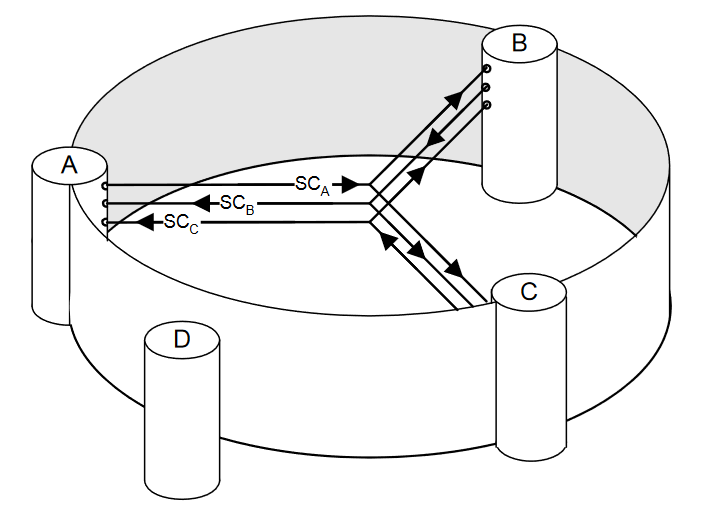
\includegraphics[width=0.85\textwidth]{images/MACsec_CA.PNG}
	\caption[Modell der MACsec Connectivity Association]{In dieser Abbildung werden 3 Stationen gezeigt, die sich in eine Connectivity Association befinden und mittels Secure Channel kommunizieren können.  }
	\label{img:MACsec_CA}
\end{figure}\gls{MACsec} kann eine sichere Kommunikation in einem LAN-Netzwerk bereitstellen. Um das \gls{MACsec} Protokoll verwenden zu können, muss jeder Nutzer eine \gls{SecY} und eine \gls{KaY} benutzen. Eine \gls{SecY} ist eine Instanz des \gls{MACsec} Protokolls, die alle Operationen ausführt, die im MACsec Standard beschrieben werden. Allerdings kann die \gls{SecY} nicht zwischen Nutzern, die das \gls{MACsec} Protokoll benutzen und normalen Nutzern unterscheiden. Um Nutzer authentifizieren zu können, wird die \gls{KaY} benötigt. Die \gls{KaY} ist für den Schlüsselaustausch, die Bereitstellung der Schlüssel, für die Autorisierung und Authentifizierung von anderen Nutzern mit einer \gls{SecY} verantwortlich. Hierfür ist ein eigener Standard, das \gls{MKA} entstanden\cite{5409813}.\\
Ein Nutzer mit einer \gls{SecY} kann in genau eine \gls{CA} eintreten. \gls{CA} bilden sichere Umgebungen, in denen die Mitglieder miteinander kommunizieren können. Nur die \gls{KaY} kann Nutzer innerhalb einer \gls{CA} erkennen. Eine \gls{MACsec} \gls{SecY} muss sich indes gar nicht bewusst sein, dass sie sich in einer \gls{CA} befindet. Wenn sich zwei \gls{SecY} innerhalb einer \gls{CA} befinden, so können sie über einen \glspl{SC} miteinander kommunizieren. Ein \gls{SC} wird auf 4 \glspl{SA} aufgeteilt. Jede Secure Association besitzt ihren eigenen \gls{SAK}, ein Schlüssel, der durch die \gls{KaY} bereitgestellt wird. Jede \gls{SA} wird durch einen \gls{SCI} identifiziert. Der Empfänger einer Nachricht kann durch den \gls{SCI} eine \gls{SA} erkennen, was wichtig ist, um den richtigen Schlüssel für die Entschlüsselung zu wählen.
 \ref{img:MACsec_CA} zeigt die \gls{SC} zwischen mehreren \gls{SecY} innerhalb eines \gls{CA}.
\subsection{MACsec auf Layer 2} \\
\label{sec:MACsec Layer 2}
\\
\begin{figure}
	\centering
	\includegraphics{images/MACsec_Frame.PNG}
	\caption[MACsec Rahmen]{In der Abbildung werden die Änderungen veranschaulicht, die der MACsec Standard an einem Rahmen vornimmt. Die grün und rot markierten Felder werden vom ICV geschützt. Das rote Feld beschreibt zudem das Nutzdaten Feld, welches verschlüsselt werden kann.}
	\label{img:MACsec_Frame}
\end{figure}Wie bereits erwähnt, arbeitet \gls{MACsec} auf der zweiten Ebene des \gls{OSI-Modell}s. Wird ein Paket über \gls{MACsec} verschickt, dann verändert \gls{MACsec} den Rahmen. Es wird ein zusätzliches Feld der SecTag angefügt und der Ethertype des Rahmens wird auf 0x88e5 gesetzt, den Ethertype von \gls{MACsec}. Zusätzlich wird ein \gls{ICV} nach dem Daten Feld konkateniert. Der \gls{ICV} wird durch den Message Authentication Code, der in \gls{MACsec} genutzt wird, gebildet. Als Input wird der SecTag, der Ethertype und das Daten Feld genommen,  sodass der \gls{ICV} alle wichtigen Bestandteile des Rahmens schützt. Es gibt in \gls{MACsec} mehrere Möglichkeiten, um einen Rahmen zu schützen. Man kann die Vertraulichkeit und Integrität oder nur Integrität schützen. Bei Vertraulichkeit und Integrität wird als erstes das Daten Feld verschlüsselt und dann der \gls{ICV} über den kompletten Rahmen gebildet. Wenn man nur Integrität auswählt, dann wird nur ein \gls{ICV} gebildet.
Die Änderungen am Rahmen ermöglichen \gls{MACsec} Angriffsmöglichkeiten wie Replay Angriffe und Denial of Service zu unterbinden. Außerdem lehnt MACsec Rahmen ab, die eine zu lange Übertragungszeit haben. Damit wird ein möglicher bounded receive delay unterbunden.
In der Abbildung \ref{img:MACsec_Frame} wird ein MACsec Rahmen dargestellt. Die grün und rot markierten Felder werden vom ICV geschützt. Das rote Feld zeigt die verschlüsselten Daten.
\\
\\
\textbf{MACsec SecTag}
\\
\\
\begin{figure}
	
	\centering 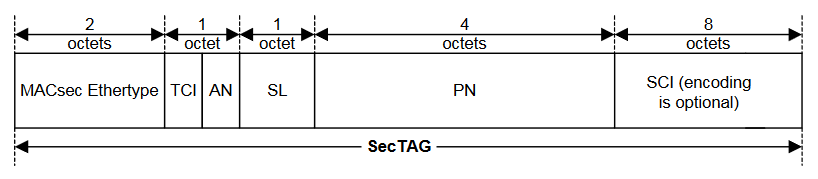
\includegraphics[width=0.9\textwidth]{images/SecTag_Format.PNG}
	\caption[SecTag Header vom MACsec Standard]{Die Abbildung zeigt den SecTag Header des MACsec Standards. Darin sind die einzelnen Felder und deren Größe in Bytes zu erkennen.}
	\label{img:SecTag}
\end{figure}Der SecTag ist ein zusätzlicher Header, der zwischen dem Ethertype Feld und dem Daten Feld eines \gls{MACsec} Rahmens eingefügt wird. Je nach Auswahl besitzt der SecTag eine Größe von 8 oder 16 Bytes und besteht aus folgenden Feldern: 
\begin{itemize}
\item dem Ethertype mit einer Größe von 2 Bytes.
\item der Tag Control Information mit einer Größe von 6 Bits.
\item der Association Number mit einer Größe von 2 Bits.
\item dem Short Field mit einer Größe von 1 Byte.
\item der Paket Nummer mit einer Größe von 4 Bytes.
\item dem SCI ein Optionales Feld mit einer Größe von 8 Bytes.
\end{itemize} \\
Ob ein Rahmen durch ein Protokoll genutzt oder verändert worden ist, kann man an dem Ethertype Feld erkennen. Bei MACsec hat das Ethertype Feld den statischen Wert 0x88E5. Darauf folgt das \gls{TCI}, das im nächsten Absatz näher erläutert wird. 
Die \gls{AN} wird mit dem Secure Channel Identifier konkateniert, um eine Secure Association zu erkennen. 
Danach kommt das Feld Short Field. Dieses Feld ist in der Regel auf 0 gesetzt. Sollte allerdings ein Paket kürzer, als die von \gls{MACsec} vorausgesetzten 48 Bytes sein, wird in diesem Feld die Länge des Pakets als Integer angegeben. 
%wird dann gepadded?
Die Paketnummer ist Teil des Initialisierungsvektors. Jedes Paket, das gesendet wird, bekommt seine eigene Paketnummer, die inkrementiert wird und somit immer unterschiedlich ist. %verweis auf den aead abschnitt
Zum Schluss kommt das optionale Feld mit dem Secure Channel Identifier. Der \gls{SCI} wird nur aktiviert, wenn das \gls{SC} Bit im \gls{TCI} gesetzt ist. Mit dem \gls{SCI} und der \gls{AN} kann man zusammen die \gls{SA} bestimmen. Das ist besonders wichtig, da jede \gls{SA} ihren eigenen \gls{SAK} besitzt. Somit muss erkannt werden, in welcher \gls{SA} die Nachricht übermittelt worden ist, um den richtigen Schlüssel zur Entschlüsselung zu benutzen. Des Weiteren wird der \gls{SCI} genutzt, um die \gls{SecY} zu identifizieren, die einen Rahmen zur Station gesendet hat. Wird kein SCI benutzt, so übermittelt das \gls{MKA} einen Wert und eine Verbindung mittels \gls{PPP} wird erstellt. In der Abbildung \ref{img:SecTag} werden die einzelnen Bestandteile eines MACsec SecTag dargstellt. Zusätzlich wird die Größe jedes Feldes in Bytes angezeigt.\\
\\
\textbf{MACsec Tag Control Information}\\
\\
\begin{figure}
	
	\centering 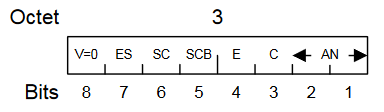
\includegraphics[width=0.65\textwidth]{images/TAG_Feld.PNG}
	\caption[Tag Control Information Feld]{In der Abbildung werden die einzelnen Bits des Tag Control Information Feldes aufgezeigt.}
	\label{img:TAG_Feld}
\end{figure}Das Tag Control Information Feld ist Bestandteil des \gls{MACsec} SecTag Headers. Das \gls{TCI} ist nur 6 Bits lang, allerdings hat jedes Bit eine feste Funktion.
Das erste Bit steht für die Versionsnummer. Im Standard wird angemerkt, dass in der Zukunft mehr als ein Bit benötigt werden, um die Versionsnummer anzuzeigen.
Das zweite Bit steht für das \gls{ES}. Das ES Bit wird nur gesetzt, wenn die ersten 6 Bytes des \gls{TCI} identisch zu den ersten 6 Bytes der MAC Adresse sind. Ist das ES Bit gesetzt, so wird vom Standard \cite{1678345} empfohlen, das SCI nicht direkt im SecTag zu kodieren und das SC Bit nicht zu setzen.
Wenn ein SCI benutzt wird, ist das SC Bit aktiv.
Nur wenn ein MACsec Rahmen mit einem Secure Channel assoziiert wird und EPON Single Copy Broadcast capability unterstützt, dann wird das SCB Bit gesetzt.
Das E Bit ist gesetzt, wenn das Secure Payload Feld verschlüsselt werden soll.
Das letzte Bit von der \gls{TCI} ist das Changed Text Bit. Ist das E Bit gesetzt und das Changed Text Bit, so wurden erfolgreich die Nutzdaten durch die \gls{SecY} verarbeitet. Ist das E Bit gesetzt, aber das Changed Text Bit noch nicht, dann wurden die Nutzdaten noch nicht durch die SecY verändert.
In der Abbildung \ref{img:TAG_Feld} ist das 6-Bit lange TCI Feld mit seinen einzelnen Komponenten und der \gls{AN} dargestellt.
\\
\\
\textbf{MACsec Secure Data}\\
\\
Das Secure Data Feld beschreibt die Nutzdaten zwischen dem SecTag und dem ICV. Das Feld kann nicht leer sein und muss  eine Länge von mindestens 48 Bytes haben, da dies die kleinste Größe eines Rahmens im Ethernet Standard ist. Ist es kürzer, dann erfolgt die Nutzung von Padding. \\
\\
\textbf{Integrity Check Value}\\
\\
Der Integrity Check Value überprüft, ob eine Nachricht manipuliert worden ist. Im MACsec Standard ist der \gls{ICV} zwischen 8 und 16 Bytes lang, je nachdem welche Cipher Suite ausgewählt worden ist. Wenn der vom Standard empfohlene Algorithmus \gls{AES-GCM} ausgewählt ist, beträgt die Länge 16 Bytes.
\subsection{MACsec Cipher Suite}\\
\\ 
In der Cipher Suite werden alle kryptografischen Algorithmen spezifiziert, die in MACsec angewendet werden können. Zu diesem Zeitpunkt befindet sich nur \gls{AES-GCM} mit einer Schlüssellänge von 128 Bit in der Cipher Suite von \gls{MACsec}. Es ist bereits eine Erweiterung der Cipher Suite geplant, in der AES-GCM mit einer Schlüssellänge von 256 Bit hinzugefügt werden soll\cite{6047536}.
Will man einen weiteren Algorithmus zur Cipher Suite hinzufügen, so müssen folgende Bedingungen erfüllt werden:
\begin{itemize}
\item Durch den Algorithmus müssen die Parameter \gls{SCI}, Paketnummer, Source Address, Destination Address, SecTag und die Nutzdaten geschützt werden. 
\item Der Algorithmus muss sowohl Integrität als auch Vertraulichkeit schützen können. 
\item Ein Verschlüsselungsalgorithmus muss bis zu 2\textsuperscript{32} -1 mal aufrufbar sein, ohne das der \gls{SAK} gewechselt werden muss.
\end{itemize} \\
\textbf{Default Cipher Suite AES-GCM}\\
\\
Die empfohlene Cipher von MACsec ist \gls{AES-GCM} auch bekannt unter \gls{AES} im Galois Counter Mode.  %etwas über die geschichte von gcm(aes) sagen.
2007 wurde AES-GCM von der amerikanischen Bundesbehörde \gls{NIST}, die auch schon den \gls{DES} und AES standardisiert hat, ein Paper veröffentlicht, in dem AES-GCM empfohlen wurde.
Es ist eine generische \gls{AEAD} Cipher, die aus der Stromchiffre AES-CTR mit einer Blocklänge von 128 Bits besteht und aus dem Message Authentikation Code GMAC, der die \gls{ICV} von MACsec mit einer Länge von 128 Bits berechnet. Wie bereits bei \ref{sec:Authenticated Encryption with Associated Data} erwähnt, benötigt ein \gls{AEAD} Schema einen fest definierten Input, der wie folgt aussieht:\\\centerline{(C,T) =\textit{enc}(IV,M,A,K)}\\
Die Schlüssellänge von \gls{AES-GCM} ist 128 Bits lang und als Schlüssel wird der \gls{SAK} einer \gls{SA} benutzt. Die ersten 64 Bits von dem 96 Bits langen \gls{IV} bestehen aus dem SCI. Die restlichen 32 Bits bilden die iterierende Paket Number.
Der Input der \gls{AD} ist die Konkatenation der Destination Mac Adresse, der Source Mac Adresse, des SecTags und zum Schluss der Nutzdaten. Die Argumente werden auch in der genannten Reihenfolge in den Algorithmus geladen.
Unter Anderem bietet MACsec 3 Möglichkeiten an, um eine Nachricht zu schützen:\\
1. Wenn MACsec nur die Integrität einer Nachricht sichern soll, dann ist der Input der Nachricht(M) leer. Die restlichen Parameter werden wie oben beschrieben als Input genommen. Die Secure Data(C) ist in diesem Fall unverändert und es folgt ein 128 Bit langer \gls{ICV}, der die Nachricht schützt.\\
2. Wenn Vertraulichkeit und auch Integrität einer Nachricht geschützt werden sollen, dann muss man einmal unterscheiden, ob man die Nachricht mit einem confidentiality offset oder ohne confidentiality offset verschlüsseln möchte.\\
2.1 Wird mit einem confidentiality offset verschlüsselt, dann wird ein fest auswählbarer Wert z.B. 30 Bytes von der Nachricht (M) nicht verschlüsselt, sondern nur mittels Integrität geschützt. Also die ersten Bytes von der Nachricht direkt nach dem SecTag sind in Klartext verfügbar, werden aber trotzdem durch den \gls{ICV} geschützt. Der Teil der Nachricht, der nicht zum confidentiality offset gehört, wird normal verschlüsselt, ist aber nicht durch den ICV geschützt. Die Secure Data ist der confidentiality offset konkateniert mit den chiffrierten Nutzdaten. \\
2.2 Wird ohne confidentiality offset verschlüsselt, dann wird das gesamte Nutzdaten Feld chiffriert. Die \gls{AD} wird wie oben beschrieben behandelt.
 %diagramm zu ad machen mit option auf confidentiality offset. 
\section{Softwareoptimierung}
Softwareoptimierungen sind angepasste Implementationen, sodass die bestehenden Hardware Unterstützungen von Systemen besser genutzt werden können, um dadurch eine Performance Steigerung zu erreichen. Es gibt Hardware Unterstützungen, die besonders nützlich für Verschlüsselungsalgorithmen sind. Das liegt daran, dass sich die CPU Instruktionen besonders gut dafür eignen, um die verwendeten mathematische Operationen in Verschlüsselungsalgorithmen zu berechnen. Viele Chiffren machen von Software Optimierungen Gebrauch und der AES Verschlüsselungsalgorithmus besitzt sogar einen eigenen Hardware Befehlssatz namens \gls{AES-NI}. In diesem Abschnitt wird daher ein Übersicht über die gängigsten Hardware Unterstützungen geschaffen, die von Verschlüsselungsalgorithmen benutzt werden.
\subsection{AES-NI}
Wie bereits erwähnt, verfügt der Verschlüsselungsalgorithmus \gls{AES} über einen eigenen Befehlssatz AES New Instructions kurz \gls{AES-NI}. Die Befehlssatzerweiterung ist seit 2010 in x86-Prozessoren zu finden. Damit werden 7 zusätzliche Assemblerbefehle unterstützt, die unter anderem Befehle für eine Verschlüsselungsrunde, eine Entschlüsselungsrunde und der Schlüsselgenerierung von AES unterstützt. In \cite{gueron2010intel} wird außerdem gezeigt, dass durch AES-NI die Performance um das 2-3 Fache gesteigert werden kann. Es wird sogar geschildert, dass AES-NI die Sicherheit von AES erhöhen kann, da durch die Instruktionen side-channel Schwächen in der Software von AES verringert werden.
\subsection{SSE}
Eine weitere wichtige Befehlssatzerweiterung ist die \gls{SSE}. SSE bringt 70 Befehlsinstruktionen mit sich und wurde bereits 1999 in x86-Prozessoren unterstützt. Aufgrund der Verwendbarkeit der Instruktionen ist der Befehlssatz in fast jedem x86-Prozessor verfügbar und seitdem sind sogar mehrere Nachfolger von SSE wie z.B SSE2 oder AVX erschienen. In SSE gibt es bis zu 16 128-Bit große Register, die über Vektor Operationen manipuliert werden können. Das hat zur Folge, dass mehrere Befehle an einem Register gleichzeitig durchgeführt werden können. Aus diesem Grund hängt es von der Parallelisierbarkeit des Verschlüsselungsalgorithmus ab, wie sehr die Chiffre vom Befehlssatz profitieren kann\cite{Ankele2016SoftwareBO}.
\subsection{AVX}
Die Advanced Vector Extensions Befehlssatzerweiterung AVX ist wie bereits erwähnt ein Nachfolger von \gls{SSE}. Bei AVX wurden die 16 128-Bit Register auf 16 256-Bit Register mit neuen Instruktionen erweitert. Das Prinzip bleibt das gleiche. Es können mit Vektor Operationen parallel mehrere Befehle an einem Register ausgeführt werden. Durch die 256-Bit großen Register können doppelt so viele Daten simultan verarbeitet werden\cite{mosnavcekoptimizing}.

%%% Local Variables:
%%% TeX-master: "diplom"
%%% End:

\chapter{AEAD Algorithmen}
\label{sec:AEAD Algorithmen}


% Ist das zentrale Kapitel der Arbeit. Hier werden das Ziel sowie die
% eigenen Ideen, Wertungen, Entwurfsentscheidungen vorgebracht. Es kann
% sich lohnen, verschiedene Möglichkeiten durchzuspielen und dann
% explizit zu begründen, warum man sich für eine bestimmte entschieden
% hat. Dieses Kapitel sollte - zumindest in Stichworten - schon bei den
% ersten Festlegungen eines Entwurfs skizziert werden.
% Es wird sich aber in einer normal verlaufenden
% Arbeit dauernd etwas daran ändern. Das Kapitel darf nicht zu
% detailliert werden, sonst langweilt sich der Leser. Es ist sehr
% wichtig, das richtige Abstraktionsniveau zu finden. Beim Verfassen
% sollte man auf die Wiederverwendbarkeit des Textes achten.

% Plant man eine Veröffentlichung aus der Arbeit zu machen, können von
% diesem Kapitel Teile genommen werden. Das Kapitel wird in der Regel
% wohl mindestens 8 Seiten haben, mehr als 20 können ein Hinweis darauf
% sein, daß das Abstraktionsniveau verfehlt wurde.
\\
In diesem Abschnitt werden verschiedene AEAD Algorithmen vorgestellt. Daraufhin werden aus den Algorithmen Kandidaten ausgewählt, die vielversprechende Ergebnisse aufweisen. Die ausgewählten Kandidaten werden detaillierter analysiert und erläutert.
\section{CAESAR Competition}\\
\\
Am 5. Juli 2012 wurde von Daniel J. Bernstein ein rundenbasierter kryptografischer Wettbewerb namens \gls{CAESAR} gestartet, um eine alternative AEAD Chiffre zum weit verbreiteten \gls{AES-GCM} zu finden \cite{bernstein2014caesar}. Im Ausschuss, der über die Verschlüsselungsalgorithmen berät, sitzen neben Bernstein auch andere Spezialisten wie z.B. Joan Daemen oder Vincent Rijmen. Beide haben den Rijndael-Algorithmus konstruiert, der später vom Nist weltweit als Standard namens \gls{AES} gewählt worden ist und in fast jedem netzwerkfähigen Gerät benutzt wird. Auch Bernstein hat mit Chacha20-Poly1305 eine weit verbreitete Chiffre, die bereits oft eine Alternative zu AES-GCM bietet. Das besondere an der CAESAR Competition ist, dass es erstmals eine standardisierte Hardware API gibt, auf dem jeder Algorithmus getestet werden kann. So können leichter Vergleiche zwischen den Chiffren auf der gleichen Plattform gezogen werden und die Ergebnisse erlangen eine größere Relevanz.
Die eingereichten Algorithmen sollten den Galois Counter Mode in mindestens einem von 3 Anwendungsfällen übertreffen.
Die Anwendungsfälle sind wie folgt definiert: 
\begin{enumerate}
\item Lightweight Applications 
\item High Performance Applications
\item Defense in Depth
\end{enumerate}
Chiffren, die für Anwendungfall 1 eingereicht werden, sollten sehr effizient auf 8-Bit \glspl{CPU} arbeiten. Trotzdem sollten die Algorithmen nicht gegenüber Side-Channel Attacks anfällig sein.\\
Anwendungsfall 2 beschreibt Chiffren die eine sehr gute Leistung auf 64-Bit \gls{CPU}s erbringen können. Außerdem sollten diese Algorithmen ebenfalls effizient auf 32-Bit CPUs sein, die hauptsächlich in Handys verbaut werden.\\
In dem letzten Anwendungsfall soll das Sicherheitsziel der Authentizität dennoch gewährleistet werden, obwohl der Initialisierungsvektor mehrfach mit dem gleichen Schlüssel benutzt worden ist. In diesem Fall spricht man auch von einem Missbrauch des Initialisierungsvektors.
Eine genaue Beschreibung der Anwendungsfälle ist in einer Email von einem der Ausschussmitglieder des \gls{CAESAR} Wettbewerbs Daniel J. Bernstein zu finden\footnote[1]{https://groups.google.com/forum/#!topic/crypto-competitions/DLv193SPSDc}.
Die \gls{CAESAR} Competition durchläuft seit 2012 mehrere Runden und hat im März 2018 7 Finalisten bekanntgegeben. Aus diesen 7 Finalisten wird ein Portfolio an Algorithmen erstellt, die von dem Gremium, in den verschiedenen Anwendungsfällen empfohlen werden.
\subsection{Finalisten des CAESAR Wettbewerbs}\\
\\
Bei dem CAESAR Wettbewerb wurden über 50 unterschiedliche \gls{AEAD} Algorithmen in der ersten Runde eingereicht. Da Experten der Kryptografie im Gremium sitzen, sind alle Finalisten mögliche Kandidaten, die in \gls{MACsec} implementiert werden können. Deshalb werden in diesem Abschnitt die Finalisten in alphabetischer Reihenfolge kurz zusammengefasst.\\
\\
ACORN: 
ACORN wurde von Hongjun Wu eingereicht und ist für den Anwendungsfall 1 konfiguriert worden. Es ist eine Stromchiffre, welche auf einem linear rückgekoppelten Schieberegister mit einer Größe von 293 Bits basiert. Der Verschlüsselungsalgorithmus wurde so entworfen, dass die Chiffre besonders effizient auf Hardware läuft. Wegen der Parallelisierbarkeit von ACORN ist der Algorithmus auch verhältnismäßig schnell in Software\cite{ACORN}.
\\
\\
AEGIS:
AEGIS basiert auf der Rundenfunktion von \gls{AES}\footnote[2]{Es ist nicht die letzte Rundenfunktion gemeint.}. Die Stromchiffre wurde von Bart Preneel\footnote[3]{Bart Preneel als auch Hongjun Wu sind beide Auschussmitglieder von der CAESAR Competition.} und Hongjun Wu veröffentlicht und kann einen sehr hohen Durchsatz erzielen. Sie wird deshalb für Anwendungsfall 2 empfohlen. Die Rundenfunktion von AEGIS wird je nach Auswahl 5 bis 8 mal wiederholt und liegt damit unter den 10 Wiederholungen, die bei AES mit einer Schlüssellänge von 128-Bit üblich sind. Aufgrund der Ähnlichkeit zu AES kann AEGIS auf die Hardware Unterstützung \gls{AES-NI} zurückgreifen\cite{AEGIS}.
\\
\\
Ascon:
Ascon wurde von Christoph Dobraunig, Maria Eichlseder, Florian Mendel und Martin Schläffer konstruiert. Durch die Struktur von Ascon und einer Ressourcen schonenden Rundenfunktion ist Ascon auf Anwendungsfall 1 spezialisiert und gehört zu den hardware optimierten Stromchiffren\cite{Ascon}.\\
\\
COLM:
COLM\footnote[4]{Die Autoren von Colm sind: Elena Andreeva, Andrey Bogdanov, Nilanjan Datta, Atul Luykx, Bart Mennink, Mridul Nandi, Elmar Tischhauser, Kan Yasuda} ist einer von 2 Finalisten, die für Anwendungsfall 3 ausgewählt wurden. Es ist eine Blockchiffre, die ebenfalls wie AEGIS auf der Rundenfunktion von AES aufgebaut ist\cite{COLM}.\\
\\
Deoxys-II:
Ein weiterer Algorithmus von den Finalisten, der auf den Missbrauch des Initialisierungsvektors spezialisiert ist. Veröffentlicht wurde Deoxys-II von: Jérémy Jean, Ivica Nikolić, Thomas Peyrin und Yannick Seurin. Ähnlich wie bei COLM basiert auch Deoxys-II auf der AES Rundenfunktion und kann somit auch von der \gls{AES-NI} Hardware Unterstützung profitieren\cite{Jean2016}.\\
\\
MORUS:
MORUS ist eine Stromchiffre, die von Hongjun Wu und Tao Huang eingereicht worden ist.
Morus ist schnell auf der Hardware, da nur hardwarefreundliche Operationen wie AND und XOR in der Rundenfunktion vom Algorithmus verwendet werden. Der Algorithmus erreicht ebenfalls gute Resultate in der Software, weil Morus  effizient mit den \gls{SSE} Instruktionen implementiert werden kann. Daher wird Morus für den Anwendungsfall 2 empfohlen\cite{wuauthenticated}.  \\
\\
OCB:
Ein weiterer schneller Verschlüsselungsalgorithmus ist von Ted Krovetz und Phillip Rogaway für den Anwendungsfall 2 vorgeschlagen worden. OCB orientiert sich an dem \gls{AES} Verschlüsselungsverfahren und nutzt infolgedessen die Rundenfunktion von AES. Die Chiffre ist in \cite{rfc7253} standardisiert worden. Der Standardisierungsprozess von OCB hatte sich verzögert, da Verfahren, die im Algorithmus benutzt wurden, patentiert sind. Mittlerweile ist es erlaubt, OCB zu benutzen unter der Bedingung, dass entweder die GNU General Public License verwendet oder die Chiffre nicht kommerziell benutzt wird\cite{krovetz2016ocb}.
\subsection{Weitere vielversprechende AEAD Algorithmen}\\
\\
NORX:
NORX wurde für die Hardware als auch für die Software optimiert. Die Cipher wurde von Jean-Philippe Aumasson, Philipp Jovanovic und Samuel Neves konstruiert. Der Grund, weshalb NORX hardwarefreundlich ist, kann man auf die genutzten Operationen im Algorithmus zurückführen. Es werden  ausschließlich XORs, ANDs ,SHIFTs und Rotationen benutzt. NORX kann durch die \gls{SSE} Instruktionen sehr effizient in Software implementiert werden. Als nicht generische Chiffre wurde NORX auch in die \gls{CAESAR} Competition eingereicht. Allerdings ist NORX nach der zweiten Runde ausgeschieden\cite{aumasson2015norx}.\\
\\
ChaCha20-POLY1305:
Die von Daniel J. Bernstein erstellte Chiffre wurde bereits in RFC7539 standardisiert.
CHACHA20-POLY1305 ist ein generisches \gls{AEAD} Verschlüsselungsverfahren. Es besteht aus der Stromchiffre ChaCha20 und dem Poly1305 MAC. ChaCha20 ist eine verbesserte Variante von der ebenfalls von Bernstein konstruierten Salsa20 Chiffre. Im Gegensatz zu \gls{AES} ist ChaCha20 nicht anfällig gegenüber timing attacks. Zudem ist ChaCha20 bis zu dreimal schneller, wenn das unterliegende System keine \gls{AES-NI} Hardware Unterstützung besitzt\cite{bernstein2008chacha}.
Der Message Authentikation Code Poly1305 wurde als erstes in Kombination mit AES als AEAD Algorithmus benutzt. Poly1305-AES bietet eine höhere Sicherheit und ist wesentlich schneller als andere bekannte generische AEAD Algorithmen wie z.B AES in Kombination mit CBC-MAC\cite{10.1007/11502760_3}.
%(ChaCha20Poly1305 Sicherheitsbeweis basiert auf dem von AES. Mit anderen Worten um ChaCha20Poly1305 zu brechen, muss man AES brechen können.)http://cr.yp.to/mac.html\\
\section{CAESAR Performance Analyse}
\\
\\
Alle Algorithmen des \gls{CAESAR} Wettbewerbs werden veröffentlicht, damit andere Spezialisten die Algorithmen auf Schwächen und Performance analysieren können. Daher wurden diverse wissenschaftliche Artikel zu dem Wettbewerb publiziert, in denen die Sicherheit oder Performance der einzelnen Algorithmen untersucht worden ist.
\subsection{Software Benchmarking}
\label{sec:software benchmarking}
In \cite{Ankele2016SoftwareBO}
wurden alle Kandidaten aus der 2. Runde, darunter auch die Finalisten, der \gls{CAESAR} Competition, analysiert. Bei der genutzten Benchmarksoftware wurde nur die Software Performance getestet. Demnach werden die Clockzyklen von einer \gls{CPU} gezählt, die benötigt werden, um eine Operation eines Verschlüsselungsalgorithmus auszuführen. Zudem werden unterschiedlich große Nachrichten und \gls{AD} verschlüsselt, um möglichst unterschiedliche und reale Bedingungen zu simulieren. 
In der Publikation wird insbesondere darauf eingegangen, welche Auswirkungen Befehlssätze auf unterschiedliche Verschlüsselungsalgorithmen haben. So wird unter anderem erwähnt, dass aufgrund der vielen \gls{AES}-basierten Algorithmen die Performance durch den \gls{AES-NI} Befehlssatz im Schnitt um das 2-3 Fache auf der Softwareebene gesteigert werden kann.
Von den Autoren gibt es kein Fazit, welche Chiffre am besten abgeschnitten haben. Vielmehr stellen sie eine Übersicht bereit, lassen jedoch die Ergebnisse weitestgehend  unkommentiert. Sie weisen lediglich darauf hin, dass die Chiffren, die software-optimierte Implementationen besitzen, wesentlich bessere Ergebnisse erzielen. Gleichwohl fällt es auf, dass die \gls{CAESAR} Finalisten AEGIS und MORUS durchschnittlich die besten Resultate erreichen. Das MORUS so hervorragende Ergebnisse erzielt ist überraschend, da MORUS eine Chiffre ist, die das Hauptaugenmerk auf die Hardwareoptimierung gelegt hat.
\\
\\
\textbf{SUPERCOP}\\
\\
\gls{SUPERCOP} ist ein Benchmarking Toolkit für kryptographische Chiffren und wurde bereits in mehreren Projekten wie eBASH\footnote[5]{ECRYPT Benchmarking of All Submitted Hashes}, eBASC\footnote[6]{ECRYPT Benchmarking of Stream Ciphers}, eBAEAD\footnote[7]{ECRYPT Benchmarking of Authenticated Ciphers}verwendet. Da auch eingereichte \gls{CAESAR} Chiffren von den Autoren in SUPERCOP hinzugefügt werden müssen, besitzt SUPERCOP eine außerordentlich große Bibliothek an Verschlüsselungsalgorithmen zum Testen\cite{bernstein2009supercop}. Um genaue Ergebnisse zu erreichen nutzt SUPERCOP den Time Stamp Counter, ein 64-Bit Register, das die Anzahl der \gls{CPU} Takte zählt. Wenn ein Test gestartet wird, so wird das Register auf 0 gesetzt und zählt die CPU Takte bis der Algorithmus beendet wird. Die Tests wurden auf unterschiedlichen Plattformen untersucht und sind in \cite{CryptoList} aufzufinden.
Hier spiegeln sich die Resultate aus\cite{Ankele2016SoftwareBO} wieder. Die softwareoptimierten Implementationen der Algorithmen erreichen weitaus bessere Ergebnisse als ohne Optimierung.


\subsection{Hardware Benchmarking}
\\
\\
Ein großes Problem bei Benchmarking von Hardware ist die Unterschiedlichkeit der Plattformen. Es gibt keine einheitliche Übereinstimmung auf welcher Hardware eine Chiffre getestet wird. Somit sind zwei kryptographische Algorithmen nicht miteinander vergleichbar, falls sie auf unterschiedlichen Systemen mit unterschiedlicher Hardware und anderen Hardware Unterstützungen getestet wurden. Die \gls{CAESAR} Competition bietet eine Hardware \gls{API} an, wodurch der Aufwand, um die verschiedenen Algorithmen auf der gleichen Plattform zu vergleichen, wesentlich vereinfacht wird. 
In  \cite{8383893} wurden alle CAESAR Kandidaten aus der dritten Runde auf der gleichen Hardware mittels der von CAESAR zur Verfügung gestellten Hardware \gls{API} getestet. Dabei wurde ein Zynq-7000 \gls{SoC} mit zwei ARM Cortex-A9, ein programmierbaren Xilinx FPGA und ein AXI Interface verwendet. 
Um die Resultate besser nachvollziehen zu können, wurde neben den 11 CAESAR Kandidaten aus der 3. Runde eine zusätzliche "dummy1" Chiffre implementiert, die hauptsächlich aus einer simplen XOR Funktion besteht. Dadurch wird der Hardware Overhead vom Präprozessor, Postprozessor und weiteren Hardwarekomponenten gemessen. In den Ergebnissen wird eine Übersicht über die Geschwindigkeit, der benötigte Speicher während der Berechnung und Stromverbrauch auf der Hardware bereitgestellt. Beim Vergleichen fällt auf, dass AEGIS128L durchaus viel Speicher im Vergleich zu anderen Chiffren  benötigt, aber AEGIS128L dafür auch der schnellste Verschlüsselungsalgorithmus ist. Dazu kommt, dass die Algorithmen, die ungefähr die gleiche Performance in Geschwindigkeit erreichen,einen höheren Stromverbrauch und mindestens genauso viel Speicher benötigen.
\section{Ausgewählte Verschlüsselungsalgorithmen}
\\
\\
\begin{table}
\adjustbox{max width=\textwidth}{
	 \begin{tabular}{ccccccc}
	Algorithmus & Schlüssellänge & IV Länge & Blockgröße & Patentfrei & Anwendungsfall & Softwareoptimierung \\
	\hline 
	ACORN-128 v3 & 128 & 128 & 128 & Ja & 1 & x \\ 
	AEGIS128L v1.1 & 128 & 128 & 128 & Ja & 2 & AES-NI \\  
	Ascon-128 v1.2 & 128 & 128 & 64 & Ja & 1 & x \\ 
	COLM v1 & 128 & 64 & 128 & Nein & 3 & AES-NI \\ 
	DEOXYS-II-128-128 v1.14 & 128 & 128 & 120 & Ja & 3 & AES-NI \\ 
	MORUS1280-128 v2 & 128 & 128 & x & Ja & 2 & SSE, AVX \\  
	OCB-128-128 & 128 & 128 & x & Nein & 2 & AES-NI, SSE \\  
	NORX-32-4-1 & 128 & 128 & x & Ja & 1 & AVX,AVX2 \\ 
	ChaCha20-Poly1305 & 256 & 96 & x & Ja & x & AVX2 \\ 
	AES-GCM & 128 & 96 & 128 & Ja & x & AES-NI \\ 
	\end{tabular}}
	\caption[Übersicht von Verschlüsselungsalgorithmen]{In der Tabelle findet man eine Übersicht der empfohlenen Algorithmen aus der CAESAR Competition mit den von den Autoren
	 vorgeschlagenen Parametern.} 
	\label{img:Eigenschaften}
\end{table}
Das Ziel der Arbeit ist, mögliche Algorithmen für MACsec zu finden, die in den Kategorien Durchsatz, Latenz oder \gls{CPU} Auslastung bessere Resultate als \gls{AES-GCM} erzielen. Daher sind die Algorithmen vom Anwendungsfall 2 in der \gls{CAESAR} Competition besonders vielversprechend. Da diese für 64-Bit-Architekturen optimiert worden sind und heutzutage 64-Bit-Architekturen am meisten verbreitet sind.
Es wurden AEGIS128L und MORUS640 von den CAESAR Finalisten ausgewählt. Laut \ref{sec:software benchmarking} gehören MORUS640 und AEGIS128L zu den schnellensten Chiffren von den Finalisten. Außerdem können beide Chiffren sehr effizient in Software implementiert werden, da AEGIS128L von der \gls{AES-NI} Hardware Unterstützung profitieren kann und MORUS640 ist gut parallelisierbar, weil MORUS640 umso mehr von der \gls{SSE} Hardware Unterstützung profitiert. 
Ebenso wurde ChaCha20Poly1305 ausgesucht. Dieser generische \gls{AEAD} Algorithmus genießt bereits große Beliebtheit und wird bereits als effiziente Alternative benutzt. In der Tabelle \ref{img:Eigenschaften} findet man eine Übersicht über die vorgestellten Algorithmen und deren Eigenschaften. Des Weiteren werden in der Tabelle auch die Hardware Unterstützungen aufgelistet, die der jeweilige Algorithmus benutzt, um seine Performance zu verbessern.
Im nächsten Abschnitt werden die 3 ausgesuchten Algorithmen detaillierter erläutert.
\subsection{AEGIS}
\label{sec:aegis}
\\
\\
AEGIS ist eine Stromchiffre, die von Hongjun Wu und
Bart Preneel veröffentlicht worden ist.
Für AEGIS wurden 3 verschiedene Varianten vorgestellt AEGIS128L, AEGIS128 und AEGIS256. Alle 3 Implementationen sind für den Anwendungsfall 2 vorgeschlagen worden, wobei laut den Autoren AEGIS128L die schnellste von den 3 Implementationen ist. Die AEGIS Familie basiert auf der AES-Rundenfunktion und profitiert sowohl von den \gls{AES-NI} Instruktionen, als auch von den Möglichkeiten der Parallelisierung, die AES besitzt. Durch die weite Verbreitung von \gls{AES} werden über die Zeit neue Instruktionen wie z.B. PCLMULQDQ\footnote[8]{PCLMULQDQ ist ein übertragsfreier Multiplikationsbefehl} zu \gls{AES-NI} oder die AES-Rundenfunktion in alle x86 Prozessoren von Intel hinzugefügt. Das sind alles Vorteile, von denen auch die AEGIS Algorithmen profitieren. Zudem nutzt AEGIS neben der AES Rundenfunktion auch XORs und ANDs, welche hardwarefreundliche Operationen sind. Die Rundenfunktion\footnote[9]{Die Wiederholung findet 5 mal bei AEGIS128, 6 mal bei AEGIS256 und 8 mal bei AEGIS128L statt. } zum Aktualisieren des Zustands wird pro Variante von AEGIS unterschiedlich oft wiederholt.
\\
Im folgenden wird ein kompletter Verschlüsselungsvorgang von AEGIS128L beschrieben. AEGIS256 und AEGIS128 unterscheiden sich nur in einigen strukturellen Details und in den Wiederholungen der Rundenfunktionen voneinander.
AEGIS128L kann in 4 verschiedene Abschnitte geteilt werden:
\begin{enumerate}
\item Initialisierung: Der Initialisierungsvektor und der geheime Schlüssel werden mit fest definierten Konstanten in den internen Zustand des Algorithmus geladen. Danach wird 10 mal die Rundenfunktion durchlaufen, um den Zustand zu aktualisieren. Am Ende jeder Rundenfunktion wird der Schlüssel als auch der Initialisierungsvektor zum Zustand XORed.
\item Associated Data: In diesem Schritt wird die \gls{AD} zum internen Zustand des Algorithmus hinzugefügt. Dabei wird die \gls{AD} in diesem Vorgang nicht verschlüsselt. Wenn die \gls{AD} kein Vielfaches von 256 Bits ist, dann wird die \gls{AD} mit 0 aufgefüllt.
\item Verschlüsselung: In diesem Abschnitt findet die eigentliche Verschlüsselung statt. Es werden zwei\footnote[10]{In AEGIS128 und AEGIS256 wird nur ein 16-Byte großer Nachrichtenblock verschlüsselt.} 16-Bytes große Nachrichtenblöcke mit dem Bitstrom, der aus dem internen Zustand von AEGIS generiert wird, XORed. Daraus entsteht das Chiffrat. Im Anschluss wird der Nachrichtenblock ein weiteres Mal mit dem internen Zustand XORed, um den Zustand bis zum nächsten Verschlüsselungsschritt zu aktualisieren. Auch hier werden die Nachrichten mit 0 aufgefüllt, sollte ein Nachrichtenblock kürzer als 16-Byte sein.
\item Finalisierung: Als letztes wird der Message Authentication Code an die Nachricht konkateniert. Dies wird bewerkstelligt, indem die Rundenfunktion von AEGIS durchlaufen wird, um den Zustand zu aktualisieren. Anschließend wird die Länge von der \gls{AD} und der Nachricht zum Zustand XORed. Dann wird ein Block aus dem internen Zustand entnommen und als Tag an die Nachricht angeheftet.
\end{enumerate} 
Die Entschlüsselung von AEGIS funktioniert genau wie die Verschlüsselung, nur das anstelle des Nachrichtenblocks, das zu entschlüsselnde Chiffrat als Input genommen wird.\\
Laut den Autoren benötigt AEGIS nur die Hälfte der Berechnungszeit von \gls{AES-GCM}. Außerdem kann durch den Designansatz der Tag ohne großen Mehraufwand berechnet werden. Obwohl AEGIS auf der AES Rundenfunktion aufbaut, kann trotzdem eine höhere TAG Sicherheit erreicht werden, als die von AES-GCM. Trotz einer gründlichen Analyse von möglichen Angriffen auf AEGIS gibt es zum jetzigen Zeitpunkt noch keinen Sicherheitsbeweis von AEGIS. Nichtsdestotrotz ist AEGIS als Finalist der \gls{CAESAR} Challenge ausgewählt worden. Deshalb kann man davon ausgehen, dass die Chiffre noch nicht gebrochen worden ist und die Experten aus der Kommission noch keinen Angriff gefunden haben, um die Sicherheit von AEGIS signifikant zu verringern.\cite{10.1007/978-3-662-43414-7_10}\cite{mosnavcekoptimizing}
\subsection{MORUS}
\\
\\
Die Stromchiffre MORUS wurde von Hongjun Wu und Tao Huang entwickelt. Von dem MORUS Algorithmus gibt es 3 verschiedene Varianten, deren Parametersets in Größe des Zustandsraums und Schlüsselgröße unterscheiden. In diesem Algorithmus gibt es eine Aktualisierungsfunktion, die mit den \gls{SSE} Instruktionen optimiert werden können. Dadurch erreicht MORUS eine geringere cpb\footnote[11]{Clock cycles per byte. Das ist eine Einheit,  um die Performance eines Algorithmus zu darzustellen} als \gls{AES-GCM}. In MORUS werden nur logische Gatter wie XOR, AND und bitweise Verschiebungen genutzt. Diese Designentscheidung macht MORUS zu einer Hardware schonenden Chiffre. MORUS besitzt den gleichen strukturellen Aufbau wie AEGIS. Abgesehen von der Aktualisierungsfunktion für den internen Zustand unterscheiden sich MORUS und AEGIS nur in Details in der Initialisierung und Finalisierung. Aus diesem Grund wird die Beschreibung eines Verschlüsselungsvorgangs nicht wiederholt. Es werden 5 Register\footnote[12]{Die Registergröße unterscheidet sich je nach Variante. MORUS640 nutzt 128-Bit große Register und MORUS1280 256 große Register.}benutzt. Das Prinzip ist hier das gleiche wie bei AEGIS. Es gibt einen geheimen internen Zustand, der mittels der Rundenfunktion aktualisiert wird. Während des Verschlüsselungsvorgangs werden \glqq Schlüssel\grqq{}-Blöcke aus dem geheimen internen Zustand generiert und mit den Nachrichtenblöcken bitweise addiert. Das Ergebnis ist der verschlüsselte Nachrichtenblock.  \\
Folgende Vorteile werden von den Autoren der MORUS Chiffren hervorgehoben: MORUS ist einer der schnellsten \gls{AEAD} Algorithmen ohne auf das Design der \gls{AES} Rundenfunktion zu setzen. Dies hat zur Folge, dass MORUS plattformübergreifend eine konstante Performance aufweist. Außerdem wird mit MORUS640-128 ein Algorithmus angeboten, der durch seine geringen Zustandsgröße auch für niedrige Bit-Architekturen geeignet ist. Zudem können MORUS und AEGIS eine stärkere Sicherheit des Message Authentikation Codes als \gls{AES-GCM} garantieren. Ein weiterer Vorteil ist, dass mit dem Design des Algorithmus der Message Authentikation Code ohne großen Aufwand berechnet werden kann.
Auch für MORUS existiert noch kein formaler Beweis, der die Sicherheit des Algorithmus bestätigt\cite{wuauthenticated}\cite{mosnavcekoptimizing}.
\subsection{ChaCha20-Poly1305}
\label{sec:chacha20-poly1305}
\\
\\
Chacha20-Poly1305 ist ein generischer AEAD Verschlüsselungsalgorithmus. Der Algorithmus besteht aus den beiden Bausteinen ChaCha20, eine Stromchiffre und den Message Authentikation Code Poly1305. ChaCha20-Poly1305 gewinnt an zunehmender Beliebtheit, da die Chiffre unabhängig von der Plattform eine konstant gute Performance aufweisen kann. Der Entwickler der unterliegenden generischen Primitive ist Daniel J. Bernstein, der 2008 zum ersten Mal eine verbesserte Variante von Salsa20, genannt ChaCha20, vorstellte\cite{bernstein2008chacha}. Kurz vorher hat er ein wissenschaftliches Dokument über Poly1305 in der Kombination mit \gls{AES}, genannt Poly1305-AES \cite{10.1007/11502760_3}, veröffentlicht, in der Bernstein seinen Message Authentikation Code vorstellt.
2015 wurde ChaCha20-Poly1305 von Google in \cite{rfc7539} standardisiert mit dem Gedanken, eine effiziente Alternative zu AES bieten zu können \cite{AdamLangley} \footnote[13]{In \cite{AdamLangley} war noch von Salsa20 die Rede. In Laufe der Zeit scheint man sich für ChaCha20 entschieden zu haben.}. Einen formalen Sicherheitsbeweis kann man unter \cite{procter2014security} finden.
ChaCha20-Poly1305 verfolgt den Encrypt-then-MAC Ansatz und benutzt einen 256-Bit langen Schüssel mit einem 96-Bit langen Initialisierungsvektor.
Im Anschluss wird die Nachricht von ChaCha20 mit dem gleichen Schlüssel, einem \gls{IV} und einen Counter verschlüsselt.
Sobald die Nachricht verschlüsselt ist, bildet Poly1305 den Tag wie folgt: Aus dem 256 langem Bit Schlüssel wird ein Schlüssel für den Poly1305 Authentikator gebildet. Poly1305 nutzt zwar einen 256 Bit langen Schlüssel, der Tag von Poly1305 ist allerdings nur 128-Bit lang.  
Poly1305 verlangt einen fest definierten Input, der diese Reihenfolge besitzen muss:
\begin{enumerate}
\item Associated Data 
\item Mittels Padding wird die Nachricht mit 0 wird auf ein Vielfaches von 16 aufgefüllt.
\item Ciphertext
\item Die Länge der Associated Data
\item Die Länge der Nachricht
\end{enumerate}
Wenn dieser Vorgang abgeschlossen ist, dann wird der Tag berechnet. Hierbei wird eine Nachricht in Vielfache von 16-Bytes geteilt. Die Blöcke werden nun als Zahl interpretiert und mittels little-endian gelesen. Jeder einzelne Block wird nun um ein Bit vergrößert. Mathematisch gesehen ist das eine Addition von $2^{128}$. Ist bis zu diesem Zeitpunkt der Nachrichtenblock nicht 17 Bytes lang, so wird Padding benutzt\footnote[14]{Es mit wird mit 0 aufgefüllt. Dadurch das die Bytes mittels little-endian gelesen werden, ändert das Padding nichts an dem eigentlichen Wert der Nachricht.}. Die Blöcke werden iterativ mit dem Zwischenergebnis addiert\footnote[15]{Der erste Block wird mit 0 addiert}. Wenn dieser Vorgang abgeschlossen ist, wird das Ergebnis mit r mod $2^{130}-5$ multipliziert. Als letzter Schritt wird das Ergebnis mit dem Wert s\footnote[16]{r und s sind Variablen, die als Resultat der Schlüsselgenerierung, gebildet werden} bitweise addiert \cite{rfc7539}.
%\cleardoublepage

%%% Local Variables:
%%% TeX-master: "diplom"
%%% End:

%
\textbf{Vorüberlegungen}
\\
\\
Die ausgewählten Kandidaten ChaCha20-Poly1305, AEGIS128L und MORUS640 sind bereits in der Linux Krypto API vertreten. 
Das bedeutet, dass die Chiffren mit crypto\_alloc\_aead im MACsec Modul initialisiert werden können.
Trotzdem müssen eine Vielzahl an Änderungen beachtet werden. Das MACsec Modul muss einen Verschlüsselungsalgorithmus mit den richtigen Parametern initialisieren. Daher müssen mit den Funktionen aus der AEAD Cipher API. 

Des Weiteren wurde in der Bachelorarbeit versucht, ACORN128 in die Kryptobibliothek vom Linux Kernel hinzuzufügen. Allerdings stellt die Bachelorarbeit nicht genügend Zeit zur Verfügung, um Chiffren in die Linux Kryptobibliothek einzufügen und nebenbei das MACsec Modul zu erweitern. Deshalb wurde aus Zeitgründen die Arbeit an ACORN128 abgebrochen.


\\
\\
\textbf{MACsec in Linux}
\\
\\
Obwohl die Publikation des MACsec Sicherheitsstandards bereits 2006 erschienen ist, wurde die Implementation des Standards  erst 2016 in den Linux-Kernel aufgenommen. Einen Überblick über den strukturellen Aufbau des MACsec Treibers wird von der Autorin des Standards Sabrina Dubroca in \cite{dubroca} gegeben. 
Wird ein Rahmen über MACsec gesendet, so wird die Funktion macsec\_start\_xmit aufgerufen. In dieser Funktion wird sowohl der komplette Prozess der Verschlüsselung als auch die Modifizierung des Rahmens durch MACsec an kleinere Teilfunktionen dirigiert. Die Funktion übernimmt 2 Parameter, einen Socket Buffer sk\_buff mit dem bis zu 64.000 Bytes große Nachrichten verschickt werden können und ein net\_device mit dem die SecY initialisiert wird. Im Verlauf von macsec\_start\_xmit wird die macsec\_encrypt Funktion aufgerufen. Dort wird die entscheidende Verschlüsselung vorbereitet und ausgeführt.
Erhält MACsec ein Rahmen, so wird die Funktion macsec\_handle\_frame aufgerufen. In dieser Funktion wird der Rahmen auf mögliche Änderungen überprüft. Je nach Sicherheitseinstellungen wird ein Paket abgewiesen oder weiter bearbeitet. Aber auch wenn eine zu große Zeitspanne zwischen dem Senden und dem Erhalten des Rahmens vergangen ist, wird die Nachricht abgewiesen. Erst nach einem erfolgreichen Abschluss aller Überprüfungen erfolgt die Entschlüsselung der Methode macsec\_decrypt.
\\
\\

Zudem wurden im Laufe der Bachelorarbeit sowohl MORUS als auch AEGIS in die Kryptobibliothek vom Linux Kernel aufgenommen. Des Weiteren wurde in der Bachelorarbeit versucht, ACORN128 in die Kryptobibliothek vom Linux Kernel hinzuzufügen. Allerdings stellt die Bachelorarbeit nicht genügend Zeit zur Verfügung, um Chiffren in die Linux Kryptobibliothek einzufügen und nebenbei das MACsec Modul zu erweitern. Deshalb wurde aus Zeitgründen die Arbeit an ACORN128 abgebrochen.

es ist erfreulich, dass diese Algorithmen Familie bereits in \cite{mosnavcekoptimizing} in den Linux Kernel implementiert worden ist.





\begin{figure}[ht]
\begin{minipage}[h]{0.45\linewidth}
\centering
\includegraphics[width=\textwidth]{images/Bild.jpg}
\caption{default}
\label{fig:sample1}
\end{minipage}
\hspace{0.5cm}
\begin{minipage}[h]{0.45\linewidth}
\centering
\includegraphics[width=\textwidth]{images/Bild.jpg}
\caption{default}
\label{fig:sample2}
\end{minipage}
\begin{minipage}[h]{0.45\linewidth}
\centering
\includegraphics[width=\textwidth]{images/Bild.jpg}
\caption{default}
\label{fig:sample3}
\end{minipage}
\hspace{0.5cm}
\begin{minipage}[h]{0.45\linewidth}
\centering
\includegraphics[width=\textwidth]{images/Bild.jpg}
\caption{default}
\label{fig:sample4}
\end{minipage}
\end{figure}

\chapter{Implementation}
\label{sec:implementation}
\lstset{escapeinside={<@}{@>}}
% Hier greift man einige wenige, interessante Gesichtspunkte der
% Implementierung heraus. Das Kapitel darf nicht mit Dokumentation oder
% gar Programmkommentaren verwechselt werden. Es kann vorkommen, daß
% sehr viele Gesichtspunkte aufgegriffen werden müssen, ist aber nicht
% sehr häufig. Zweck dieses Kapitels ist einerseits, glaubhaft zu
% machen, daß man es bei der Arbeit nicht mit einem "Papiertiger"
% sondern einem real existierenden System zu tun hat. Es ist sicherlich
% auch ein sehr wichtiger Text für jemanden, der die Arbeit später
% fortsetzt. Der dritte Gesichtspunkt dabei ist, einem Leser einen etwas
% tieferen Einblick in die Technik zu geben, mit der man sich hier
% beschäftigt. Schöne Bespiele sind "War Stories", also Dinge mit denen
% man besonders zu kämpfen hatte, oder eine konkrete, beispielhafte
% Verfeinerung einer der in Kapitel 3 vorgestellten Ideen. Auch hier
% gilt, mehr als 20 Seiten liest keiner, aber das ist hierbei nicht so
% schlimm, weil man die Lektüre ja einfach abbrechen kann, ohne den
% Faden zu verlieren. Vollständige Quellprogramme haben in einer Arbeit
% nichts zu suchen, auch nicht im Anhang, sondern gehören auf Rechner,
% auf denen man sie sich ansehen kann.

In Kapitel 3 wurde begründet, welche Algorithmen für die Implementation in den Sicherheitsstandard ausgewählt wurden. Im Folgenden wird erklärt, auf welchem aktuellen Stand sich die \gls{MACsec} Implementierung auf dem Linux Kernel befindet und welche Änderungen an dem bestehenden Quellcode gemacht werden müssen, um weitere Algorithmen hinzuzufügen.

\section{Linux}\\
\\ 
Linux ist ein Betriebssystem, welches maßgeblich von Linus Torvalds geprägt worden ist. Eine Besonderheit an Linux ist, dass es von mehreren Unternehmen weiterentwickelt wird, die regelmäßig das bestehende Betriebssystem erweitern, indem neue Versionen für das Betriebssystem und austauschbare Linux-Kernel veröffentlicht werden.\\
Ein Linux-Kernel ist das Herzstück des Betriebssystems und stellt Schnittstellen für die Software bereit, um auf die Hardware eines Systems zugreifen zu können\footnote[17]{Die unterschiedlichen Kernel-Versionen, die von Linux unterstützt werden, sind unter kernel.org aufzufinden.}.\\
\\
\textbf{Linux Krypto API}
\\
\\
Die Linux Kernel Application Programming Interface ist eine Programmierschnittstelle, die durch den Linux-Kernel bereitgestellt wird. Mit der Linux Krypto API haben Kernel Treiber wie MACsec Zugriff auf alle Verschlüsselungsalgorithmen, die durch den Linux-Kernel unterstützt werden. Außerdem überprüft die Linux Krypto API das System und kann somit automatisch die softwareoptimierten Implementationen der Verschlüsselungsalgorithmen auswählen, falls das unterliegende System Hardware Unterstützungen anbietet. Es werden unterschiedliche "{}Cipher APIs"{} angeboten für verschiedene Algorithmentypen:
\begin{itemize}
\item Blockchiffren
\item Stromchiffren
\item AEAD Algorithmen
\item Hash Funktionen
\item Zufallszahlengeneratoren
\end{itemize} Damit ein Verschlüsselungsalgorithmus erfolgreich aufgerufen werden kann, muss ein transformation object (tfm) initialisiert werden. Das tfm ist eine Instanz der Implementation eines Verschlüsselungsalgorithmus.
Oft wird so ein Objekt auch "{}Cipher Handle{}" genannt.
Ein Aufruf eines Verschlüsselungsalgorithmus muss somit folgende Schritte absolvieren. 
\begin{enumerate}
\item Initialisierung eines tfm
\item Anwendung der Verschlüsselungsoperation
\item Zerstörung des tfm
\end{enumerate}
Jede Cipher API stellt eigene Funktionen zur Verfügung, um ein tfm zu initialisieren und auszuführen. 
Im Folgenden werden die wichtigsten Funktionen aus der AEAD Cipher API vorgestellt, die in MACsec Verwendung finden:
\begin{itemize} 
\item crypto\_alloc\_aead initialisiert die Cipher Handle.
\item crypto\_free\_aead zerstört die Cipher Handle.
\item crypto\_aead\_ivsize gibt den Initialisierungsvektor zurück.
\item crypto\_aead\_authsize konfiguriert die Größe des Tags.
\item crypto\_aead\_setkey konfiguriert den Schlüssel und Schlüssellänge.
\item crypto\_aead\_encrypt startet die Verschlüsselung.
\item crypto\_aead\_decrypt startet die Entschlüsselung.
\item aead\_request\_set\_crypt nimmt die zu verschlüsselnden/entschlüsselnden Daten entgegen und konkateniert die Daten intern hinter die AD.
\item aead\_request\_set\_tfm allokiert Speicher für das tfm.
\item aead\_request\_set\_ad konfiguriert die Größe der AD.
\end{itemize} Wie bereits erwähnt, muss als erstes ein tfm initialisiert werden. Dafür wird die Funktion crypto\_alloc\_aead aufgerufen, die mit einem String den richtigen Algorithmus auswählt und initialisiert. Doch bevor es zu einer korrekten Anwendung der Verschlüsselungsoperation kommen kann, müssen einige Vorbereitungen gemacht werden. Es muss die crypto\_aead\_setkey Funktion aufgerufen werden. Damit wird der Cipher Handle die Schlüssellänge und der zu nutzende Schlüssel mitgeteilt. Ebenfalls muss die Tag Größe mit der crypto\_aead\_setauthsize Funktion definiert werden. In dem MACsec Modul werden diese Vorbereitungen direkt nach der Initialisierung in der Funktion macsec\_alloc\_tfm umgesetzt.\\
Nachdem Schlüssel und Tag konfiguriert worden sind, muss der Speicher für die Cipher Handle allokiert werden. Normalerweise wird hierfür die aead\_request\_alloc Funktion aufgerufen, die ein tfm entgegennimmt und automatisch den Speicher allokiert. Da das MACsec Modul mit unterschiedlich großen Nachrichten arbeitet und die Nachrichtengröße ebenfalls in die Allokation mit einbezogen werden muss, wird in der Funktion macsec\_alloc\_req der benötigte Speicher errechnet und anschließend mit aead\_request\_set\_tfm allokiert. \\
Erst jetzt ist es möglich, die zu verschlüsselnden/entschlüsselnden Daten für den Algorithmus bereitzustellen. Die MACsec AEAD Cipher API nutzt für die zu bearbeitenden Daten eine Speicherstruktur namens scatter-gather Liste. Die scatter-gather Liste setzt Pointer auf die Daten. Das erleichtert den Umgang mit größeren Datenmengen, da nur eine scatter-gather Liste mit den Pointern übergeben werden muss.
In aead\_request\_set\_crypt werden die scatter-gather Liste, der Initialisierungsvektor und die Länge der Nachricht an den Verschlüsselungsalgorithmus übergeben. 
Außerdem wird noch die Länge der AD benötigt. Das wird mit der Funktion aead\_request\_set\_ad umgesetzt.
In aead\_request\_set\_callback wird eine Funktion entgegengenommen, die aufgerufen wird, wenn die der Verschlüsselungsvorgang/ Entschlüsselungsvorgang beendet wird.
Erst wenn diese Vorbereitungen abgeschlossen sind und alle Funktionen aufgerufen worden sind, ist es möglich, die Verschlüsselungsoperation mit crypto\_aead\_encrypt oder crypto\_aead\_decrypt zu starten.
Das MACsec Modul hat seine eigene Verschlüsselungsfunktion namens macsec\_encrypt in der viele Maßnahmen präpariert werden, um eine erfolgreiche Verschlüsselung durchführen zu können. Neben der Ausführung der AEAD Cipher API Funktionen muss MACsec in der macsec\_encrypt und macsec\_decrypt den Initialisierungsvektor bilden, den Header des Rahmens gemäß der MACsec Definitionen aus \ref{sec:MACsec Layer 2} verändern und die scatter-gather Liste initialisieren \cite{kerneldoc} \cite{mosnavcekoptimizing}.
\section{MACsec Kernel Modul}\\
\\
Obwohl die Publikation des MACsec Sicherheitsstandards bereits 2006 erschienen ist, wurde die Implementation des Standards  erst 2016 in den Linux-Kernel aufgenommen. Einen Überblick über den strukturellen Aufbau des \gls{MACsec} Treibers wird von der Autorin des Standards Sabrina Dubroca in \cite{dubroca} gegeben. Wird ein Rahmen über MACsec gesendet, so wird die Funktion macsec\_start\_xmit aufgerufen. In dieser Funktion wird sowohl der komplette Prozess der Verschlüsselung als auch die Modifizierung des Rahmens durch MACsec an kleinere Teilfunktionen dirigiert. Die Funktion übernimmt 2 Parameter, einen Socket Buffer sk\_buff mit dem bis zu 64.000 Bytes große Nachrichten verschickt werden können und ein net\_device mit dem die SecY initialisiert wird. Im Verlauf von macsec\_start\_xmit wird die macsec\_encrypt Funktion aufgerufen. Dort wird die entscheidende Verschlüsselung vorbereitet und ausgeführt.
Erhält \gls{MACsec} ein Rahmen, so wird die Funktion macsec\_handle\_frame aufgerufen. In dieser Funktion wird der Rahmen auf mögliche Änderungen überprüft. Je nach Sicherheitseinstellungen wird ein Paket abgewiesen oder weiter bearbeitet. Aber auch wenn eine zu große Zeitspanne zwischen dem Senden und dem Erhalten des Rahmens vergangen ist, wird die Nachricht abgewiesen. Erst nach einem erfolgreichen Abschluss aller Überprüfungen erfolgt die Entschlüsselung der Methode macsec\_decrypt.
\section{iproute2}
\\
\\
iproute2 ist ein Linux Werkzeug, dass zurzeit von Stephen Hemminger bearbeitet wird. Intern nutzt iproute2 einen Linux Service namens netlink, um mit den Netzwerkstack des Kernels zu kommunizieren. Für die Konfiguration von MACsec bietet iproute2 eine Reihe von Befehlen an, die unter \cite{Manpage} zu finden sind. Mit der aktuellen Implementierung kann man bei iproute2 den Verschlüsselungsalgorithmus von \gls{MACsec} auswählen. Mittels dem Optional Cipher besteht die Möglichkeit, \glqq default\footnote[18]{Wenn default ausgewählt wird, dann wird automatisch \gls{AES-GCM} mit einer Schlüssellänge von 128 Bits verwendet.}\grqq{} und \glqq aes-gcm-128\grqq{} auszuwählen. Um mehrere Algorithmen nutzen zu können, muss das iproute2 erweitert werden, damit die hinzugefügten Algorithmen auswählbar und von MACsec erkannt werden.\\ Allerdings treten dabei drei essentielle Probleme in der aktuellen Implementierung auf:
\begin{enumerate}
\item Die MACsec Cipher Suite unterstützt nur einen Algorithmus. 
\item Die derzeitige \gls{SecY} im \gls{MACsec} Modul kann nicht erkennen, welcher Algorithmus benutzt wird. Um zwischen verschiedenen Algorithmen auswählen zu können, muss daher die SecY von MACsec erweitert werden.
\item Das aktuelle MACsec Modul im Linux Kernel ist  statisch programmiert und genau auf die Parameter von AES-GCM-128 angepasst. Daher muss die Implementierung dynamischer gestaltet werden, da nicht alle Verschlüsselungsalgorithmen genau die gleichen Parameter von \gls{AES-GCM} verwenden.
\end{enumerate}\\
\\
Die \gls{MACsec} Cipher Suite ist eine Liste von statischen Variablen und Structs, in denen Parameter, die MACsec vom Verschlüsselungsalgorithmus verlangt, definiert werden.
Die Erweiterung der Cipher Suite ist daher simpel, da nur eine statische Variable mit einer einzigartigen Identifikationsnummer für den hinzugefügten Algorithmus erstellt werden muss.\\
\\
\textbf{iproute2 Schnittstelle}\\
\\
Mit dem Cipher Optional wird ein String entgegen genommen. Daraufhin überprüft das iproute2, ob es zu dem String eine Identifikationsnummer aus der Cipher Suite von MACsec gibt. Ist das der Fall, so wird die Identifikationsnummer an das \gls{MACsec} übermittelt. 
\section{MACsec Erweiterung}
\\
\\
\begin{figure}
  \lstset{language=C}
  \begin{lstlisting}
  struct macsec_secy {
	struct net_device *netdev;
	unsigned int n_rx_sc;
	sci_t sci;
	u16 key_len;
	u16 icv_len;
	enum macsec_validation_type validate_frames;
	bool operational;
	bool protect_frames;
	bool replay_protect;
	u32 replay_window;
	struct macsec_tx_sc tx_sc;
	struct macsec_rx_sc __rcu *rx_sc;
	<@\textcolor{red}{u64 csid;}@>
	};
  \end{lstlisting}
  \caption[Abbildung der SecY]{\acrshort{MACsec} Die Felder der Security Entity. Die Änderung an der Security Entity wurde mit rot markiert.}
\label{lst:macsec_SecY}
\end{figure}Als ein großes Problem in der Programmierung stellte sich heraus, dass \gls{MACsec} kategorisch unterschiedliche Algorithmen mit anderen Parametersätzen wie z.B. einer anderen Schlüssellänge als 128-Bit ablehnt. Zum einen liegt das daran, dass MACsec eine Reihe von Sicherheitsvorkehrungen hat, die vor der Initialisierung eines Algorithmus genau überprüfen, ob die Schlüssellänge exakt mit den Parametern von \gls{AES-GCM}-128 übereinstimmen. Die Sicherheitsüberprüfungen sind so komplex, dass noch keine Möglichkeit gefunden wurde, Algorithmen mit größeren Schlüsseln dynamisch in MACsec zu implementieren, ohne dabei die Sicherheit von \gls{MACsec} zu gefährden. 
Zum anderen wurden in der aktuellen Implementation z.B. die Länge des Initialisierungsvektors mit einer statischen Variable der Länge von 12-Bytes definiert. Deshalb wurden alle Vorkommen der statischen Variable mit einer Funktion namens crypto\_aead\_ivsize() aus der Linux Kryptographie Bibliothek ausgetauscht. Die Funktion erkennt die initialisierte Chiffre und gibt die Länge des Initialisierungsvektors aus. In einigen Methoden muss Speicherkapazität für die Parameter allokiert werden. So wird garantiert, dass egal welcher Algorithmus benutzt wird, die richtige Größe des Initialisierungsvektors allokiert wird.
Um Algorithmen mit einem variablen Initialisierungsvektor in MACsec unterstützen zu können, muss zudem der SecTag vergrößert werden, da der Initialisierungsvektor ein Bestandteil vom SecTag ist. Somit wird der SecTag um 4 Byte vergrößert, damit \gls{MACsec} auch Algorithmen unterstützen kann, die einen Initialisierungsvektor mit einer Länge von 16-Bytes benötigen.
\subsection{SecY Erweiterungen}\\
\\
Um mehrere Algorithmen auswählen zu können, muss die Security Entity von Macsec erweitert werden. Die \gls{SecY} von MACsec wird mit der Funktion macsec\_changelink\_common initialisiert. In dieser Funktion werden die Parameter von der iproute2 Konfiguration an die SecY von MACsec übergeben. Im Anschluss validiert \gls{MACsec} die überreichte Identifikationsnummer des Verschlüsselungsalgorithmus aus der Cipher Suite. Wird kein passender Algorithmus gefunden, gibt MACsec eine Fehlermeldung an den Kernel zurück. Die Identifikationsnummer wird mit dem Feld u64 csid beschrieben. 
In dieser Arbeit wurde die SecY mit der u64 csid erweitert. So ist es möglich, die Identifikationsnummer der Chiffre zu speichern. Da die SecY maßgeblich am Verschlüsselungsprozess teilnimmt, kann man in den entscheidenden Schritten über die Identifikationsnummer prüfen und den richtigen Parameter auswählen. Die Struktur von der SecY ist in der Abbildung \ref{lst:macsec_SecY} zu sehen.
\section{Herausforderungen}
\\
\\
Die größte Herausforderung war die Fehlersuche im Kernel Modul. Tritt im Programm ein Fehler auf, kann trotzdem ein Paket verschickt werden. Das hat zur Folge, dass fehlerhafte Pakete erst beim Validieren von dem Programm bemerkt werden, obwohl die Ursache des Problems woanders liegt. Aufgrund dieser Tatsache hat es sich als äußerst schwer herausgestellt, den Ursprung eines Fehlers zu finden. Es hat einen hohen Zeitaufwand benötigt, um einzelne Probleme zu ermitteln, da nicht direkt der richtige Ansatz zum Lösen des Problems gefunden wurde.
\subsection{MORUS640, AEGIS128L}
\\
\\
Während der Tests mit den Programmen ping und iperf3 traten in 1 Prozent der Fälle Authentifizierungsfehler bei AEGIS128L und MORUS640 auf. Die Authentifizierungsfehler kamen zustande, weil in der Entschlüsselungsfunktion ein Buffer Stream einzelne ankommende Pakete in zwei geteilt hat. Daher wurde ein Buffer Overflow in einer Streaming Methode, die beim Entschlüsseln aufgerufen wird, vermutet. Aufgrund der Tatsache, dass die beiden Algorithmen erst kürzlich zum Linux Kernel hinzugefügt worden sind\footnote[19]{\url{https://git.kernel.org/pub/scm/linux/kernel/git/torvalds/linux.git/commit/?id=3e1a29b3bf66c2850ea8eba78c59c234921c0b69}},schien es als wahrscheinlich, dass noch mögliche Fehler in der Implementierung vorhanden sind. Daher wurde der Autor der Implementation um Rat gefragt und es wurde versucht, den Fehler in der Linux Bibliothek libkcapi zu reproduzieren.
Im Nachhinein hat sich herausgestellt, dass durch die statische Programmierung von MACsec der Initialisierungsvektor unbemerkt auf 12-Bit verkleinert wurde. Das hat zu kritischen Fehlern geführt, da MORUS640 und AEGIS128L einen Initialisierungsvektor mit der Länge von 16-Bit benötigen. 
\subsection{ChaCha20-Poly1305}
\\
\\
ChaCha20-Poly1305 war der einzige Algorithmus, der sich nicht korrekt mittels crypto\_alloc\_aead initialisieren ließ. Es wurde erwähnt, dass ChaCha20-Poly1305 einen besonderen Input benötigt, um den Message Authentication Code bilden zu können\cite{rfc7539}. Daher lag die Vermutung nahe, dass die interne Datenverarbeitung von MACsec diese Struktur nicht bereitstellen kann oder stattdessen eine andere Struktur benutzt. Im Endeffekt konnte ChaCha20-Poly1305 nicht initialisiert werden, da die MACsec Cipher Suite keine Algorithmen mit einer 256-Bit Schlüssellänge unterstützt. Aus diesem Grund konnte kein gültiger \gls{SAK} generiert werden, der für die korrekte Initialisierung des Algorithmus unverzichtbar ist. Das Problem wurde mit einem statischen Schlüssel behoben. Das hat zwar Auswirkungen auf die Sicherheit von \gls{MACsec}, aber für die Performancemessungen ist dies unerheblich.  
 

%(Die SecY speichert bereits andere wichtige Parameter für die Verschlüsselungsalgorithmen wie die Schlüssellänge oder die Länge des ICV) und bietet sich somit für die Erweiterung an.
%Verwirrenderweise wird die csid in der originalen Implementation nirgends gespeichert, sondern in jeder Funktion, in der die csid benötigt wird, wird auf die Schlüssellänge der Chiffre getestet. Über die Schlüssellänge wird dann auf die csid geschlossen. Das macht Sinn wenn der Standard nur zwei Algorithmen mit unterschiedlicher Schlüssellänge unterstützt\footnote{Aktuell werden AES-GCM-128 und AES-GCM-256 unterstützt.}. Da MORUS640, AEGIS128L und AES-GCM-128 die gleiche Schlüssellänge haben, ist die Schlüssellänge keine eineindeutige Eigenschaft mehr, um einen Algorithmus zu erkennen. Daher wurde ein anderer Lösungsansatz verfolgt. In der Arbeit wurde die SecY mit der csid erweitert. Die csid wird während der Initialisierung von der SecY in der SecY gespeichert. 


%Zum Zeitpunkt des Schreibens wird vermutlich die aktuelle MACsec Implementation überarbeitet. Es sind bereits Bausteine der MACsec Erweiterung von[MAcsec Standard mit 256 Bit einfügen] im Code auffindbar. Auch die Cipher Suite von MACsec wurde bereits erweitert. Allerdings gibt es noch keine Implementierung, um AES 
\\
\\



%%% Local Variables:
%%% TeX-master: "diplom"
%%% End:

\chapter{Evaluation}
\label{sec:evaluation}


% Zu jeder Arbeit in unserem Bereich gehört eine Leistungsbewertung. Aus
% diesem Kapitel sollte hervorgehen, welche Methoden angewandt worden,
% die Leistungsfähigkeit zu bewerten und welche Ergabnisse dabei erzielt
% wurden. Wichtig ist es, dem Leser nicht nur ein paar Zahlen
% hinzustellen, sondern auch eine Diskussion der Ergebnisse
% vorzunehmen. Es wird empfohlen zunächst die eigenen Erwartungen
% bezüglich der Ergebnisse zu erläutern und anschließend eventuell
% festgestellte Abweichungen zu erklären.

Es wurden nun unterschiedliche Verschlüsselungsalgorithmen vorgestellt und in das aktuelle \gls{MACsec Modul} implementiert.
Im Folgenden werden Performance Tests durchgeführt, um zu sehen, ob dadurch eine höhere Datenübertragungsrate und niedrigere Latenz erreicht werden kann.\\
Leider war es nicht möglich, MORUS640 und AEGIS128L mit dem software-optimierten Implementationen zu testen. Die Implementationen werden erst ab dem Linux Kernel 4.18 unterstützt, der zum Zeitpunkt der Test noch nicht funktionsfähig zur Verfügung stand. Deshalb mussten die Implementationen zu einer älteren Kernel-Version hinzugefügt werden, wodurch noch keine Softwareoptimierungen unterstützt werden können. In \ref{sec:software benchmarking} wurde gezeigt, wie sehr sich die Optimierungen auf die Performance auswirken. Daher ist zu erwarten, dass die fehlenden Optimierungen negative Auswirkungen auf die Latenz und Datenübertragungsrate von MORUS640 und AEGIS128L haben.
\section{Testaufbau}\\
\\
Die Testergebnisse werden auf zwei Rechnern evaluiert, die mittels eines LAN-Kabels miteinander verbunden sind.
Auf den Rechnern läuft folgende Hardware:
\begin{table}[hp]
\centering
\begin{tabular}{cccc}
\multicolumn{2}{l}{Prozessor:} \multicolumn{2}{r}{Intel i5-4590 3.3GHz} \\ 
\multicolumn{2}{l}{RAM:} \multicolumn{2}{r}{16GB}\\ 
\multicolumn{2}{l}{Betriebssystem:} \multicolumn{2}{r}{Ubuntu 18.04 mit dem Linux-Kernel 4.15.0-32} \\ 
\end{tabular} 
\caption[Testaufbau]{In der Tabelle wird die Hardware des Systems aufgelistet.}
\end{table}\\Jeder Algorithmus wird mit verschiedenen Paketgrößen getestet, um reale Bedingungen zu simulieren.
Dabei wird geschaut, ob die unterschiedlichen Paketgrößen Auswirkungen auf die Latenz oder die Datenübertragungsrate haben. Die Datenübertragungsrate kann mit dem Werkzeug iperf3 gemessen werden. Neben der Bandbreite sind die Latenz und die CPU Auslastung entscheidende Messkriterien. Dafür bietet sich das Werkzeug ping an. Damit lässt sich die Round-trip time feststellen. Das ist die zeitliche Übertragung eines festen Pakets zum Zielrechner und die Beantwortung des Pakets vom Zielrechner.
Folgende Tests werden durchgeführt:
\begin{enumerate}
\item \gls{MACsec} wird mit den Verschlüsselungsalgorithmen \gls{AES-GCM}, ChaCha20-Poly1305 , AEGIS128L und MORUS640 mit ping getestet. Die verwendeten Paketgrößen sind 128, 256, 512, 1024, 1400 und 1514 Bytes. Die Tests werden sowohl mit Verschlüsselung als auch ohne Verschlüsselung ausgeführt.
\item MACsec wird mit den Verschlüsselungsalgorithmen AES-GCM, ChaCha20-Poly1305 , AEGIS128L und MORUS640 mit iperf3 getestet. Die verwendeten Paketgrößen sind 128, 256, 512, 1024, 1400 und 1514 Bytes. Die Tests werden sowohl mit Verschlüsselung als auch ohne Verschlüsselung ausgeführt.
\item Ethernet wird mit den Paketgrößen 128, 256, 512, 1024, 1400 und 1514 Bytes mit iperf3 und ping getestet.
\end{enumerate}
Die verwendeten Paketgrößen sind gängige Größen, um Verschlüsselungsalgorithmen zu testen. Daher werden diese Werte übernommen, um leichter Vergleiche zu anderen Arbeiten ziehen zu können.
Die Auswertungen werden mit einem Bash-Skript ausgeführt, welches auf beiden Testrechnern die Konfigurationen mit den unterschiedlichen Paketgrößen und Verschlüsselungsalgorithmen via \gls{SSH} aktualisiert und die Analyse mit ping oder iperf3 startet.
Iperf3 sendet in einem Zeitraum von 10 Sekunden Pakete an einen Server, der auf dem Empfängerrechner konfiguriert wurde und misst jede Sekunde den durchschnittlichen Datendurchsatz. Die Resultate der Testsoftware werden in eine Datei geschrieben und gespeichert. In eine Datei wird jeweils nur ein Test mit einem Verschlüsselungsalgorithmus und nur einer Paketgröße geschrieben. Im Zuge der Datenanalyse hat sich herausgestellt, dass die Daten leichter zu untersuchen sind, wenn sie sich in einer Datei befinden. Daher wurden im Nachhinein alle Dateien eines Verschlüsselungsalgorithmus mit unterschiedlichen Paketgrößen konkateniert und zu einer Datei gebündelt, was zu einer Erleichterung der Datenanalyse führte.\\
Die iperf3 Tests wurden mit \gls{AES-GCM} und ChaCha20-Poly1305 für jede Paketgröße 250 mal wiederholt. Die Evaluation von MORUS640 und AEGIS128L konnten aufgrund von Implementationsproblemen erst später durchgeführt werden und wurden aus Zeitgründen 100 mal für jede Paketgröße wiederholt. \\
Die ping Tests wurden 50000 mal für jede Paketgröße wiederholt. Normalerweise wird eine ping Anfrage in einem festen Intervall gesendet, der eine Sekunde beträgt. Mit der adaptiven ping Option kann der Testvorgang beschleunigt werden, indem die ping Anfragen sofort gesendet werden, sobald die vorherige Anfrage beantwortet wurde. 
\subsection{Datendurchsatz}
\\
\\
In Abbildung \ref{img:bytes-e} und \ref{img:bytes-we} sind die Ergebnisse der Evaluation in Diagrammen dargestellt.
Aus den Diagrammen ist ersichtlich, dass es keinen Unterschied macht, ob \gls{MACsec} die Daten verschlüsselt und dann den TAG bildet oder die Verschlüsselung auslässt und nur den TAG generiert. Das ist damit zu erklären, dass bei \gls{AEAD} Algorithmen die Verschlüsselung und Tag Bildung in der gleichen Verschlüsselungsrunde durchgeführt werden. Deshalb benötigt ein Algorithmus trotzdem die gleiche Anzahl an Zyklen, um einen TAG zu einer Nachricht zu bilden,
egal ob Verschlüsselung angewendet wird oder nicht. Des Weiteren sieht man, dass noch Verbesserungspotenzial im Vergleich zur Ethernet möglich ist, wenn ein Verschlüsselungsalgorithmus mit einer niedrigen Paketgröße ausgewählt wurde. Allerdings kann jeder Algorithmus die Leitung komplett auslasten, sobald eine Paketlänge von 1024 Bytes erreicht wird. \gls{AES-GCM} und ChaCha20-Poly1305 haben sehr ähnliche Testergebnisse. ChaCha20-Poly1305 kann also von der Performance durchaus eine Alternative zu \gls{AES-GCM} sein. MORUS640 und AEGIS128L schließen ab einer Paketlänge von 1024 Bytes mit ChaCha20-Poly1305 und AES-GCM auf. Bei niedrigen Paketlängen erreicht MORUS640 knapp die Hälfte des Durchsatzes von AES-GCM. AEGIS128L ist im Vergleich zu MORUS640 ein wenig schneller und kann bereits ab einer Paketlänge von 512 Bytes zu \gls{AES-GCM} und ChaCha20-Poly1305 aufholen. Die genauen Testresultate findet man in der Appendix in den Tabellen \ref{tab:bytes-e} und \ref{tab:bytes-we} .
\afterpage{%
\begin{figure}[!p]
\centering
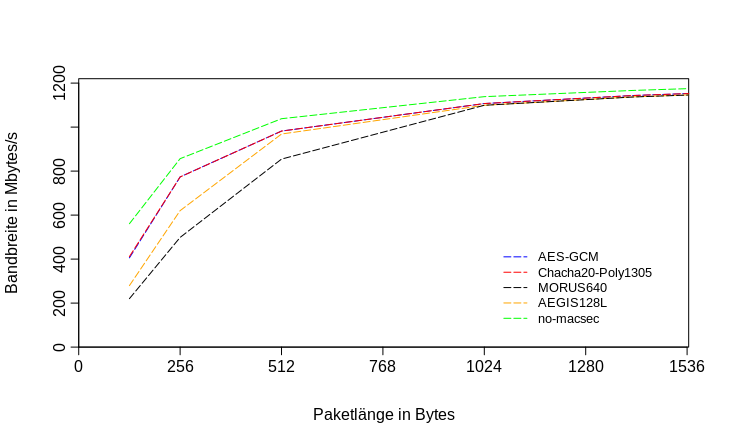
\includegraphics[width=0.95\textwidth]{images/bytese-new.png}
\caption[Bandbreite Diagramm mit aktivierter Verschlüsselung]{In dem Diagramm wird die Bandbreite der Verschlüsselungsalgorithmen in mbytes/s dargestellt. Die Test wurden mit aktivierter Verschlüsselung durchgeführt.}
\label{img:bytes-e}
\end{figure}
\begin{figure}[!p]
\centering
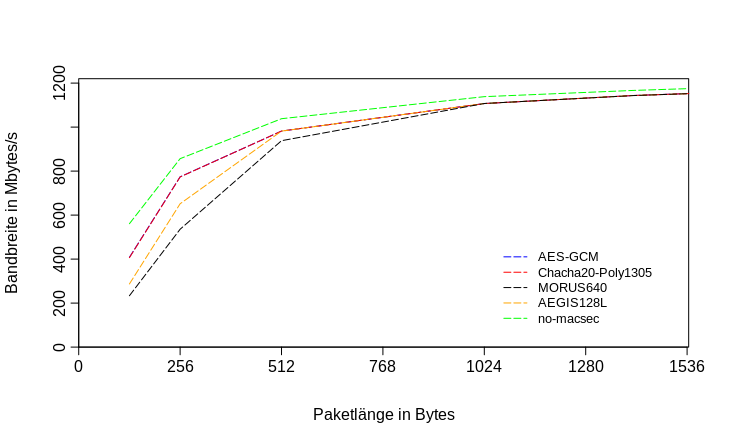
\includegraphics[width=0.95\textwidth]{images/bytes-we-new.png}
\caption[Diagramm der Bandbreite ohne Verschlüsselung]{In dem Diagramm wird die Bandbreite der Verschlüsselungsalgorithmen in mbytes/s dargestellt. Die Test wurden ohne Verschlüsselung durchgeführt.  }
\label{img:bytes-we}
\end{figure}
\clearpage
}
\subsection{CPU Auslastung}
\\
\\
Während der iperf3 Testvorgänge wurde gleichzeitig die CPU Auslastung des Computers ermittelt. Die Testergebnisse sind in den Diagrammen \ref{img:CPU-E} und \ref{img:CPU-WE} aufzufinden. Zusätzlich gibt es in der Appendix in den Tabellen \ref{tab:CPU-e} und \ref{tab:CPU-we} die genauen Resultate. Die Daten zeigen, dass alle hinzugefügten Algorithmen eine hohe \gls{CPU} Auslastung bei niedrigen Paketgrößen aufweisen. Bei MORUS640 ist ein sogenannter Bottleneck bei den Paketgrößen erkennbar. Das heißt, dass MORUS640 die CPU komplett auslastet und somit die Performance von MORUS640 durch die CPU gedrosselt wird. Die \gls{CPU} Auslastung bei MORUS640 liegt bei den Paketgrößen 128, 256 und 512 Bytes im Schnitt bei 96,8 Prozent. Die enorme Belastung der CPU in den niedrigen Paketgrößen lässt sich dadurch erklären, dass bei geringen Paketgrößen die Verschlüsselungsalgorithmen wesentlich häufiger aufgerufen werden müssen als bei großen Paketgrößen. Der häufige Funktionsaufruf führt auch bei ChaCha20-Poly1305 zu einer hohen CPU Auslastung. Diese liegt im Durchschnitt bei 96,6 Prozent, wenn eine Paketlänge von 128 benutzt wird. Einzig und allein \gls{AES-GCM} hat durchgängig eine durchschnittliche CPU Auslastung von knapp einem Prozent und liegt damit fortwährend sehr nah an der CPU Auslastung von Ethernet und erzielt in einigen Fällen sogar bessere Ergebnisse als die Ethernet. Dies lässt sich nur durch Messungenauigkeiten in den Resultaten erklären.
\subsection{Latenz}
\\
\\
Die Paketumlaufzeit ist in der Appendix in den Tabellen \ref{tab:Lat-e} und \ref{tab:Lat-we} aufzufinden.
Auch bei der Latenz weist \gls{AES-GCM} die besten Resultate auf mit einer durchschnittlichen Zeit von 0,143 ms bei einer Paketgröße von 128 Bytes und 0,147 ms bei 1514 Bytes. Die Latenz ist nur minimal größer als die von Ethernet mit 0,136 ms bei 128 Bytes und ist in einigen Fällen sogar etwas besser mit 0,15 bei 1514 Bytes. Das ist erneut durch eine Messungenauigkeit erklärbar. MORUS640 und AEGIS128L haben mit Abstand die höchste Latenz, die im Schnitt bei 0,162 ms bei AEGIS128L und 0,16 ms bei MORUS640 liegt. AEGIS128L ist somit 10 Prozent langsamer als \gls{AES-GCM} mit einer durchschnittlichen Zeit von 0,145 ms. Ein Grund dafür könnte die fehlende Software Optimierung sein. Daher wurden diese Ergebnisse, wie bereits in der Einleitung des Kapitels erwähnt, erwartet. Auffallend ist die geringe Varianz von ChaCha20-Poly1305 und AES-GCM. Die durchschnittliche Paketumlaufzeit zwischen den Paketlängen hat bei ChaCha20-Poly1305 nur eine Differenz von 0,005 ms und ist nur noch bei AES-GCM minimal geringer mit 0,004  ms. Daraus lässt sich eine konstante Performance von AES-GCM und ChaCha20-Poly1305 erkennen. Die Diagramme sind in der Appendix \ref{img:AEGISping} aufzufinden.
\afterpage{%
\begin{figure}[!p]
\centering
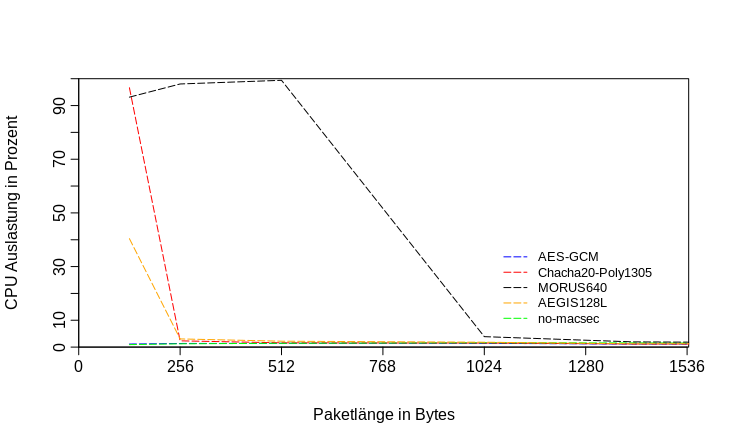
\includegraphics[width=0.95\textwidth]{images/CPU-E-NEW.png}
\caption[CPU Auslastung mit aktivierter Verschlüsselung]{Das Diagramm zeigt die CPU Auslastung in Prozent der einzelnen Verschlüsselungsalgorithmen, Während der Tests wurde die Verschlüsselung aktiviert.  }
\label{img:CPU-E}
\end{figure}
\begin{figure}[!p]
\centering
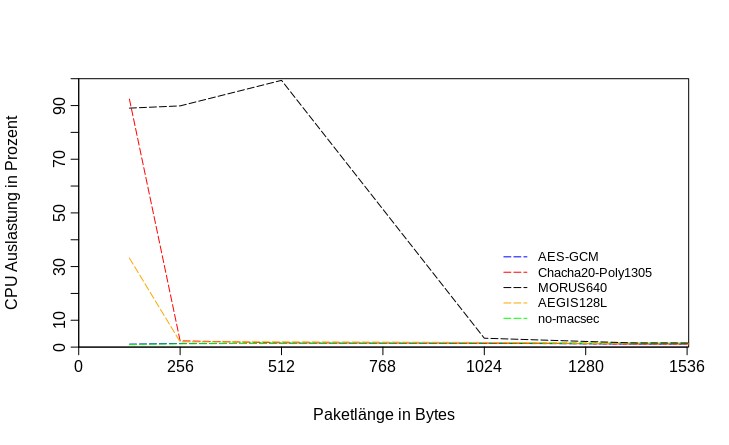
\includegraphics[width=0.95\textwidth]{images/cpu-we-new.png}
\caption[CPU Auslastung ohne Verschlüsselung]{Das Diagramm zeigt die CPU Auslastung in Prozent der einzelnen Verschlüsselungsalgorithmen, Während der Tests wurde keine Verschlüsselung verwendet. }
\label{img:CPU-WE}
\end{figure}
\clearpage
}
\section{Sicherheitsevaluation}
\label{sec:sicherheitsevalutation}
\\
\\
Der Sicherheitsstandard MACsec garantiert folgende Sicherheitsziele: Vertraulichkeit, Integrität, Authentizität, bounded receive delays und Schutz vor Replay Angriffen. Im folgenden Abschnitt wird auf die Änderungen eingegangen, die in Kapitel \ref{sec:implementation} beschrieben worden sind und ob diese Auswirkungen auf die genannten Sicherheitsmerkmale haben. Im Rahmen der Bachelorarbeit wird es nicht möglich sein, komplette Sicherheitsanalysen der einzelnen Algorithmen vorzustellen, daher werden nur die wichtigsten Kriterien behandelt. Im kompletten Abschnitt wird davon ausgegangen, dass die Algorithmen korrekt verwendet werden.
\subsection{Vertraulichkeit}
Da ein Verschlüsselungsalgorithmus maßgeblich für das Sicherheitsziel der Vertraulichkeit verantwortlich ist, muss man sehr sorgfältig überprüfen, ob die gemachten Änderungen einen Einfluss auf die Sicherheit haben.
Es wurden insgesamt 3 weitere Verschlüsselungsalgorithmen implementiert. \\
\\
\textbf{ChaCha20-Poly1305}
\\
\\
ChaCha20-Poly1305 besitzt eine Schlüssellänge von 256-Bits und ist somit doppelt so lang wie die Schlüssellänge von \gls{AES-GCM}. Desweiteren bietet ChaCha20-Poly1305 wenig Angriffsfläche gegenüber "timing-attacks", die bei \gls{AES-GCM} gefunden wurden\cite{cache-collision-timing-attacks-against-aes}. Somit kann sogar eine höhere Sicherheit der Vertraulichkeit gewährleistet werden als bei AES-GCM. An dieser Stelle muss erwähnt werden, dass die Implementation von ChaCha20-Poly1305 nur mit einem statischen Schlüssel erfolgen konnte. In diesem Fall wirkt sich der geringe Initialisierungsvektor negativ aus, da mit einem Initialisierungsvektor der Länge von 96-Bit nur ca 256 Gigabyte verschlüsselt werden können, ohne das sich der Initialisierungsvektor wiederholt\cite{rfc7539}. In Anbetracht der Tatsache, dass die Implementierung des Autors von ChaCha20-Poly1305 nur einen Prototyp darstellt, um Performance-Analysen ausführen zu können, ist die Schwächung der Sicherheit von \gls{MACsec} durch einen statischen Schlüssel vernachlässigbar, da eine korrekte Implementierung von ChaCha20-Poly1305 die Sicherheit des MACsec Moduls nicht beeinträchtigen würde.\\
\\
\textbf{AEGIS128L, MORUS640}
\\
\\
AEGIS128L und MORUS640 benutzen jeweils eine Schlüssellänge von 128-Bits. In der wissenschaftlichen Publikation von AEGIS128L\cite{10.1007/978-3-662-43414-7_10} und MORUS640\cite{wuauthenticated} ist eine genaue Sicherheitsanalyse zu den Algorithmen zu finden. Allerdings existiert noch kein formaler Sicherheitsbeweis für die beiden Algorithmen. Dies könnte daran liegen, dass die Algorithmen erst 2014 publiziert worden sind. Aus diesem Grund können AEGIS128L und MORUS640 noch nicht zu den wohluntersuchten Algorithmen gezählt werden. Das hat keine negativen Auswirkungen auf das Sicherheitsziel der Vertraulichkeit, aber bei der Anwendung von AEGIS128L und MORUS640. Dementsprechend sollte bei der Anwendung von AEGIS128L und MORUS640 weniger Vertrauen entgegengebracht werden.

\subsection{Integrität}
\\
\\
Da der Betriebsmodus \gls{AEAD} verwendet wird, wird auch Message Authentication Code ausgetauscht, sobald eine andere Chiffre verwendet wird. Deshalb muss der verwendete Message Authentication Code der einzelnen Chiffren betrachtet werden. Der Aufbau der Message Authentication Codes wurde bereits in \ref{sec:aegis} und \ref{sec:chacha20-poly1305} genauer erläutert. \\
\\
\textbf{Poly1305}
Die Nutzung von Poly1305 hat keinen negativen Effekt auf die Integrität des Sicherheitsstandards.
\\
\\
\textbf{AEGIS128L, MORUS640}
\\
\\
Trotz eines fehlenden Sicherheitsbeweises wird in \cite{10.1007/978-3-662-43414-7_10} und \cite{wuauthenticated} explizit hervorgehoben, dass AEGIS128L und MORUS640 eine 128-Bit Sicherheit für Authentikation bereitstellen können, die höher ist als die von \gls{AES-GCM}. Demzufolge wird die Sicherheit der Integrität bei der Anwendung von MORUS640 und AEGIS128L verstärkt.\\
\\
\textbf{Authentizität}
\\
\\
Da die Authentizität durch den ICV des MACsec Standards gesichert und der \gls{ICV} durch den Message Authentication Code gebildet wird, schwächt dies nicht die Authentizität, weil in diesem Abschnitt gezeigt wurde, dass ein Austausch des Verschlüsselungsalgorithmus keine negativen Auswirkungen auf die Integrität ausübt.
\subsection{Verfügbarkeit}
\\
\\
Im Sicherheitsstandard wurden nur zusätzliche Verschlüsselungsalgorithmen hinzugefügt. Diese Änderungen können Auswirkungen auf die Vertraulichkeit oder Integrität haben. Allerdings hat ein anderer Verschlüsselungsalgorithmus keinen Effekt auf die Verfügbarkeit, solange das \gls{MACsec} Modul korrekt verwendet wird und kein aktiver Angriff auf das System vorliegt. Darüber hinaus hat ein aktiver Angriff keine Auswirkungen auf die Funktionsweise des Verschlüsselungsalgorithmus.
\subsection{Replay Angriffe}
\\
\\
\gls{MACsec} schützt vor Replay Angriffen, in dem jedes versendete Paket eine Paketnummer zugeteilt bekommt, die nach jedem Paket inkrementiert wird. Wiederholt sich eine Paketnummer, so wird das Paket abgelehnt. Zwar wurden aufgrund der Paketnummer Änderungen am SecTag vorgenommen, das beschränkt sich allerdings nur auf die Vergrößerung des Paketnummer Feldes, um größere Initialisierungsvektoren zu unterstützen. Trotzdem wird der vergrößerte SecTag weiterhin komplett vom \gls{ICV} geschützt, sodass keine neuen Angriffsmöglichkeiten auf den SecTag bestehen.\clearpage
\section{Resultate}
Die Ergebnisse fallen durchmischt aus. 
ChaCha20-Poly1305 kann größtenteils bei der Bandbreite und \gls{CPU} Auslastung mit \gls{AES-GCM} mithalten. Auch bei der Latenz ist ChaCha20-Poly1305 im Schnitt nur 4,1 Prozent langsamer als \gls{AES-GCM}, was ein tolerierbarer Wert ist. Anders sehen die Ergebnisse bei AEGIS128L und MORUS640 aus. Die Daten zeigen, dass die Latenz von MORUS640 und AEGIS128L weit hinter denen von ChaCha20-Poly1305 und \gls{AES-GCM} liegen. Wenn die Bandbreite betrachtet wird, können AEGIS128L und MORUS640 bei geringen Paketgrößen auch nicht mithalten. Trotzdem muss erwähnt werden, dass Software Optimierungen große Auswirkungen auf einen Algorithmus haben können\cite{Ankele2016SoftwareBO} und sowohl AEGIS128L als auch MORUS640 zum Zeitpunkt der Experimente keinen Zugriff auf deren Optimierungen hatten. In Anbetracht dieser Tatsache fallen die Ergebnisse von MORUS640 und AEGIS128L durchaus akzeptabel aus. Insgesamt zeigt sich, dass auf dieser Testumgebung die aktuelle ChaCha20-Poly1305 Implementation durchaus eine ernsthafte Alternative zu \gls{AES-GCM} bieten kann.


%%% Local Variables:
%%% TeX-master: "diplom"
%%% End:

\chapter{Fazit}
\label{sec:Fazit}
Das Ziel dieser Arbeit war es, das \gls{MACsec} Modul mit zusätzlichen Verschlüsselungsalgorithmen zu erweitern. Dabei wurden unterschiedliche Algorithmen vorgestellt und analysiert. Anschließend wurde eine Auswahl aus den vielversprechendsten Algorithmen getroffen, die daraufhin in ein erweitertes MACsec implementiert wurden. Damit unterschiedliche Chiffren unterstützt werden, musste das Kernel Modul dynamischer gestaltet und unter anderem der SecTag vergrößert werden. Mögliche Schwächen und Sicherheitsmängel der Änderungen sind angesprochen worden. \\
Im Anschluss erfolgten die Performance Tests der einzelnen Chiffren, in dem die Latenz, Datenübertragungsrate und die Auslastung der \gls{CPU} gemessen wurden. Um einen Vergleichswert zu haben, wurden ebenfalls Messungen mit normalen Ethernet Paketen gemacht.\\
Die Ergebnisse zeigen, dass ChaCha20-Poly1305 durchaus als Alternative zu \gls{AES-GCM} genommen werden kann. Die Ergebnisse in der Bandbreite sind fast identisch und die CPU Auslastung befindet sich ebenfalls im gleichen Bereich. Nur bei der Paketumlaufzeit ist ChaCha20-Poly1305 im Durchschnitt 4 Prozent langsamer. Für einen Algorithmus, der nicht auf die \gls{AES-NI} Hardware Unterstützung setzt, ist das ein gutes Ergebnis.\\
AEGIS128L und MORUS640 haben als Algorithmen viel Potential. Die Ergebnisse in dieser Arbeit spiegeln das nicht wider. Im Gegensatz dazu erreichen AEGIS128L und MORUS640 in anderen Publikationen\cite{Ankele2016SoftwareBO} und Benchmarking Tools \cite{bernstein2009supercop} sogar bessere Ergebnisse in der Datenübertragung als \gls{AES-GCM}. Ein Grund für das schlechte Abschneiden dieser Algorithmen könnte sein, dass es nicht möglich war, die Algorithmen mit ihren Softwareoptimierungen zu testen. Daher müssen in dieser Hinsicht noch mehr Nachforschungen betrieben werden.





%%% Local Variables:
%%% TeX-master: "diplom"
%%% End:

\chapter{Appendix}
\label{sec:Appendix}
\section{Iperf3 Testergebnisse}
\makeatletter
\setlength{\@fptop}{0pt}
\makeatother
\begin{table}[hp]
\centering
\large
\begin{tabular}{c||c c c c c}
Paketgröße & Baseline & AES-GCM & AEGIS128L & ChaCha20-Poly1305 & MORUS640  \\
\hline  
in bytes & \multicolumn{4}{c}{in mbytes/s} \\
\hline 
128 & 560.89 & 405.67 & 279.42 & 411.31 & 220.18  \\ 
256 & 856.55 & 773.62 & 620.32 & 773.34 & 498.61  \\ 
512 & 1038.22 & 981.99 & 968.6 & 981.89 & 854.6 \\ 
1024 & 1138.45 & 1107.16 & 1099.26 & 1107.10 & 1099.25  \\ 
1400 & 1136.97 & 1143.71 & 1137.6 & 1143.61 & 1136.93 \\
1514 & 1145.89 & 1152.72 & 1146.48 & 1152.51 & 1145.89 \\  
\end{tabular}
\centering \caption[Datenübertragungsrate mit Verschlüsselung]{ Die Bandbreite in mbyte/s mit Verschlüsselung.}
\label{tab:bytes-e}
\end{table}

\begin{table}[hp]
\centering
\large
\begin{tabular}{c||c c c c c}
Paketgröße & Baseline & AES-GCM & AEGIS128L & ChaCha20-Poly1305 & MORUS640  \\
\hline  
in bytes & \multicolumn{4}{c}{in mbytes/s} \\
\hline
128 & 560.89 & 408.04 & 286.94 & 406.62 & 233.43  \\ 
256 & 856.55 & 774.06 & 651.54 & 773.45 & 535.74  \\ 
512 & 1038.22 & 982.04 & 1107.23 & 981.93 & 938.27 \\ 
1024 & 1138.45 & 1107.12 & 1143.69 & 1107.16 & 1107.38  \\ 
1400 & 1136.97 & 1143.67 & 1137.6 & 1143.65 & 1143.36 \\
1514 & 1145.89 & 1152.69 & 1152.1 & 1152.52 & 1152.21 \\  
\end{tabular} 
\centering \caption[Datenübertragungsrate ohne Verschlüsselung]{ Die Bandbreite in mbyte/s ohne Verschlüsselung.}
\label{tab:bytes-we}



\end{table}
\begin{table}[hp]
\centering
\large
\begin{tabular}{c||c c c c c}
Paketgröße & Baseline & AES-GCM & AEGIS128L & ChaCha20-Poly1305 & MORUS640  \\
\hline  
in bytes & \multicolumn{4}{c}{in Prozent} \\
\hline
128 & 0.91 & 1.13 & 40.39 & 96.63 & 93.13  \\ 
256 & 1.21 & 1.34 & 3.04 & 2.32 & 98.04  \\ 
512 & 1.41 & 1.4 & 2.19 & 1.58 & 99.41 \\ 
1024 & 1.60 & 1.39 & 1.81 & 1.51 & 3.88  \\ 
1400 & 1.55 & 1.11 & 1.22 & 1.16 & 1.93 \\
1514 & 1.5 & 1.11 & 1.22 & 1.15 & 1.84 \\  
\end{tabular} 
\caption[CPU Auslastung mit Verschlüsselung]{ Die CPU Auslastung in Prozent mit Verschlüsselung.}
\label{tab:CPU-e}
\end{table}
\begin{table}[htp]
\centering
\large
\begin{tabular}{c||c c c c c}
Paketgröße & Baseline & AES-GCM & AEGIS128L & ChaCha20-Poly1305 & MORUS640  \\
\hline
in bytes & \multicolumn{4}{c}{in Prozent} \\
\hline  
128 & 0.91 & 1.08 & 33.15 & 92.39 & 89.04  \\ 
256 & 1.21 & 1.35 & 1.96 & 2.32 & 89.87  \\ 
512 & 1.41 & 1.4 & 1.95 & 1.57 & 99.39 \\ 
1024 & 1.60 & 1.41 & 1.72 & 1.5 & 3.3  \\ 
1400 & 1.55 & 1.12 & 1.21 & 1.14 & 1.54 \\
1514 & 1.5 & 1.12 & 1.2 & 1.15 & 1.51 \\  
\end{tabular} 

\caption[CPU Auslastung ohne Verschlüsselung]{ Die CPU Auslastung in Prozent ohne Verschlüsselung.}
\label{tab:CPU-we}
\end{table}
\clearpage
\section{ping Testergebnisse}
\begin{table}[h]
\large
\begin{tabular}{c||c c c c c}
Paketgröße & Baseline & AES-GCM & AEGIS128L & ChaCha20-Poly1305 & MORUS640  \\
\hline  
in bytes & \multicolumn{4}{c}{in ms} \\
\hline 
128 & 0.136 & 0.143 & 0.147 & 0.149 & 0.152  \\ 
256 & 0.14 & 0.144 & 0.148 & 0.15 & 0.154  \\ 
512 & 0.142 & 0.144 & 0.161 & 0.152 & 0.16 \\ 
1024 & 0.146 & 0.146 & 0.174 & 0.153 & 0.17  \\ 
1514 & 0.15 & 0.147 & 0.181 & 0.154 & 0.177 \\
\end{tabular}
\caption[Paketumlaufzeit mit Verschlüsselung]{Die durchschnittlichen Paketumlaufzeiten mit Verschlüsselung in ms.}
\label{tab:Lat-e}
\end{table}

\begin{table}[h]
\large
\begin{tabular}{c||c c c c c}
Paketgröße & Baseline & AES-GCM & AEGIS128L & ChaCha20-Poly1305 & MORUS640  \\
\hline  
in bytes & \multicolumn{4}{c}{in ms} \\
\hline 
128 & 0.136 & 0.141 & 0.148 & 0.148 & 0.15  \\ 
256 & 0.14 & 0.145 & 0.147 & 0.148 & 0.153  \\ 
512 & 0.142 & 0.149 & 0.15 & 0.149 & 0.157 \\ 
1024 & 0.146 & 0.155 & 0.155 & 0.15 & 0.166  \\ 
1514 & 0.15 & 0.161 & 0.159 & 0.151 & 0.17 \\
\end{tabular}
\caption[Paketumlaufzeit ohne Verschlüsselung]{Die durchschnittlichen Paketumlaufzeiten ohne Verschlüsselung in ms.}
\label{tab:Lat-we}
\end{table}

\begin{figure}[!p]
\centering
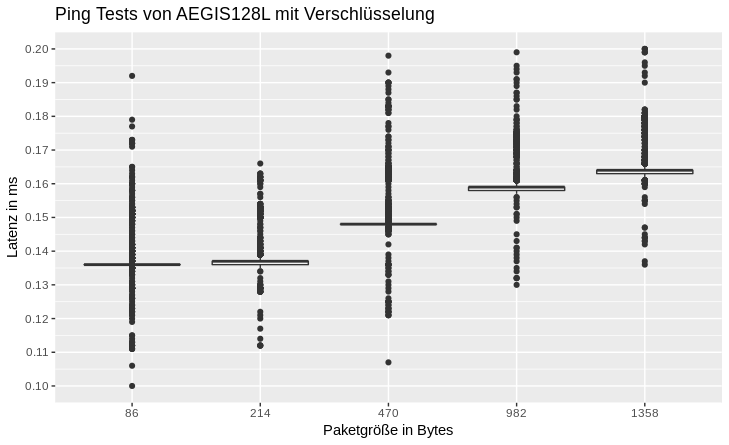
\includegraphics[width=0.95\textwidth]{images/aegiseping.png}
\caption[Ping Diagramm mit AEGIS128L mit Verschlüsselung]{Das Boxplot Diagramm zeigt die Ping Tests mit dem Verschlüsselungsalgorithmus AEGIS128L. Es wurden 50.000 Tests durchgeführt. Es wurde mit Verschlüsselung getestet. }
\label{img:AEGISping}
\end{figure}
\begin{figure}[!p]
\centering
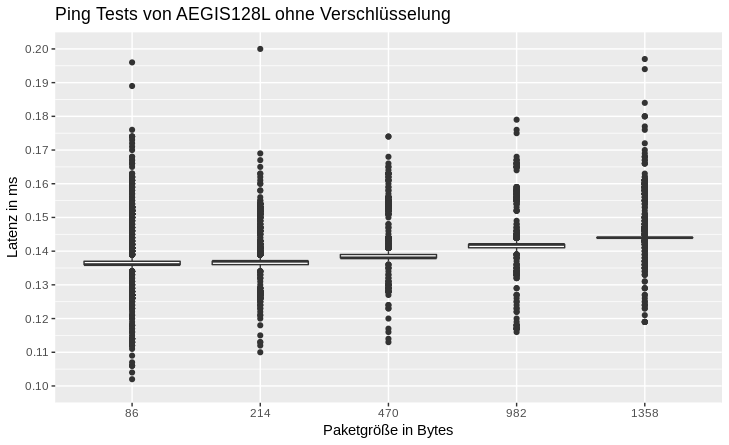
\includegraphics[width=0.95\textwidth]{images/aegisweping.png}
\caption[Ping Diagramm mit AEGIS128L ohne Verschlüsselung]{Das Boxplot Diagramm zeigt die Ping Tests mit dem Verschlüsselungsalgorithmus AEGIS128L. Es wurden 50.000 Tests durchgeführt. Es wurde ohne Verschlüsselung getestet.  }
\label{img:CPU-WE2}
\end{figure}
\begin{figure}[!p]
\centering
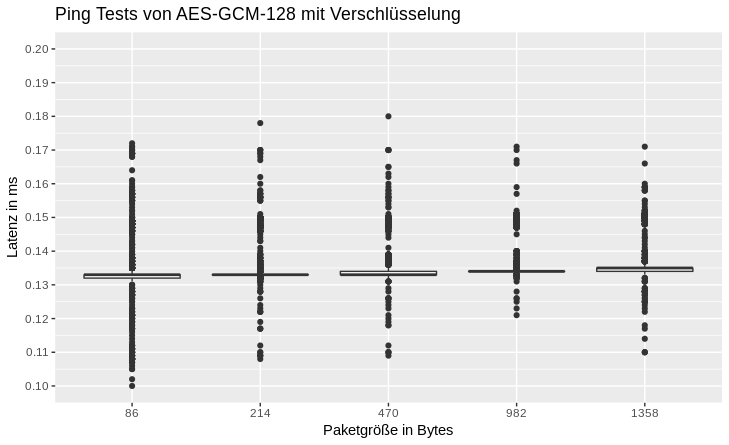
\includegraphics[width=0.95\textwidth]{images/aesEping.png}
\caption[Ping Diagramm mit AES-GCM mit Verschlüsselung]{Das Boxplot Diagramm zeigt die Ping Tests mit dem Verschlüsselungsalgorithmus AES-GCM. Es wurden 50.000 Tests durchgeführt. Es wurde mit Verschlüsselung getestet.  }
\label{img:CPU-WE3}
\end{figure}
\begin{figure}[!p]
\centering
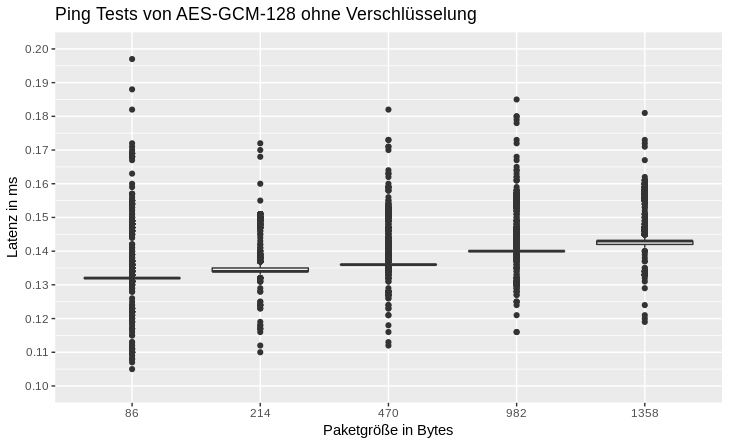
\includegraphics[width=0.95\textwidth]{images/aesWEping.png}
\caption[Ping Diagramm mit AES-GCM ohne Verschlüsselung]{Das Boxplot Diagramm zeigt die Ping Tests mit dem Verschlüsselungsalgorithmus AES-GCM. Es wurden 50.000 Tests durchgeführt. Es wurde ohne Verschlüsselung getestet.  }
\label{img:CPU-WE3}
\end{figure}
\begin{figure}[!p]
\centering
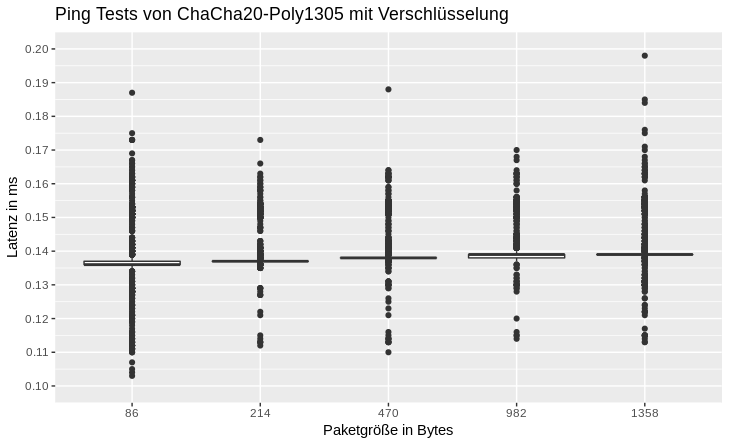
\includegraphics[width=0.95\textwidth]{images/chachaEping.png}
\caption[Ping Diagramm mit ChaCha20-Poly1305 mit Verschlüsselung]{Das Boxplot Diagramm zeigt die Ping Tests mit dem Verschlüsselungsalgorithmus ChaCha20-Poly1305. Es wurden 50.000 Tests durchgeführt. Es wurde mit Verschlüsselung getestet. }
\label{img:CPU-WE4}
\end{figure}
\begin{figure}[!p]
\centering
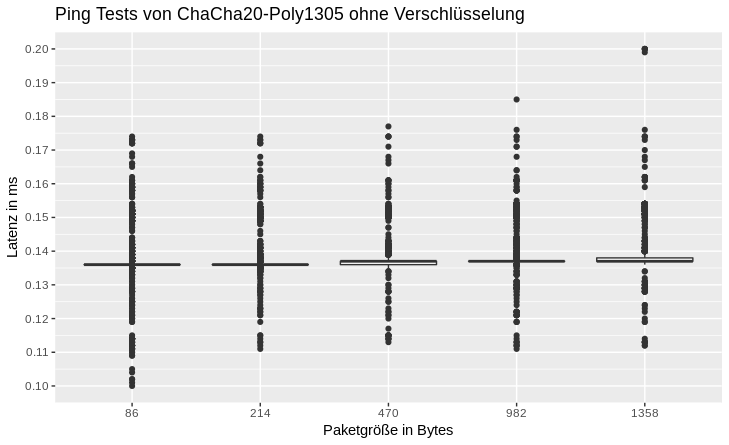
\includegraphics[width=0.95\textwidth]{images/chachaweping.png}
\caption[Ping Diagramm mit ChaCha20-Poly1305 ohne Verschlüsselung]{Das Boxplot Diagramm zeigt die Ping Tests mit dem Verschlüsselungsalgorithmus ChaCha20-Poly1305. Es wurden 50.000 Tests durchgeführt. Es wurde ohne Verschlüsselung getestet. }
\label{img:CPU-WE5}
\end{figure}
\begin{figure}[!p]
\centering
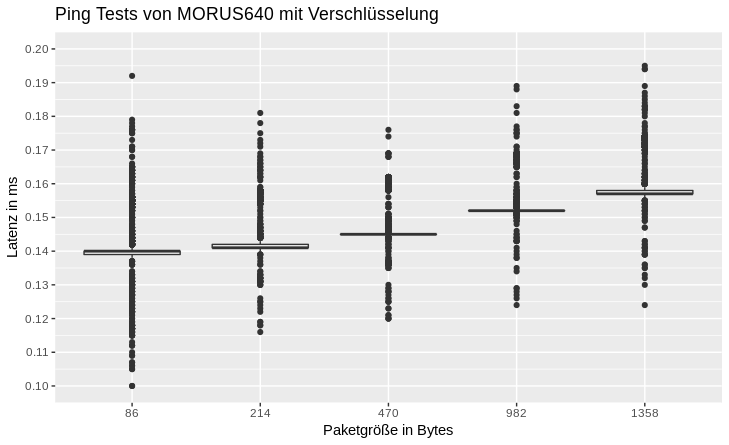
\includegraphics[width=0.95\textwidth]{images/moruseping.png}
\caption[Ping Diagramm mit MORUS640 mit Verschlüsselung]{Das Boxplot Diagramm zeigt die Ping Tests mit dem Verschlüsselungsalgorithmus MORUS640. Es wurden 50.000 Tests durchgeführt. Es wurde mit Verschlüsselung getestet.   }
\label{img:CPU-WE6}
\end{figure}
\begin{figure}[!p]
\centering
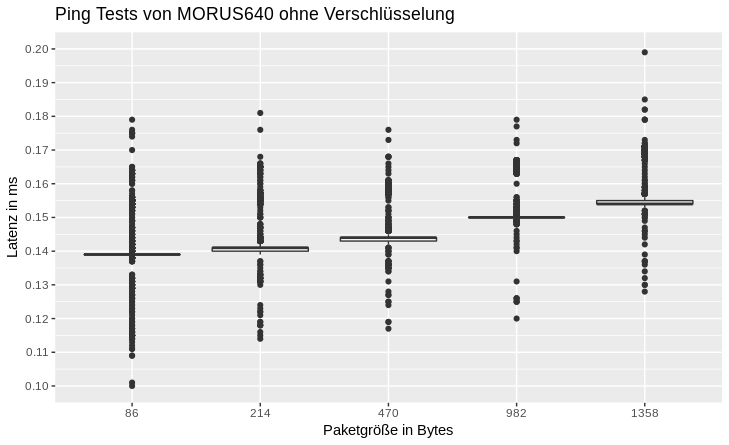
\includegraphics[width=0.95\textwidth]{images/Morusweping.png}
\caption[Ping Diagramm mit MORUS640 ohne Verschlüsselung]{Das Boxplot Diagramm zeigt die Ping Tests mit dem Verschlüsselungsalgorithmus MORUS640. Es wurden 50.000 Tests durchgeführt. Es wurde ohne Verschlüsselung getestet.  }
\label{img:CPU-WE7}
\end{figure}
\begin{figure}[!p]
\centering
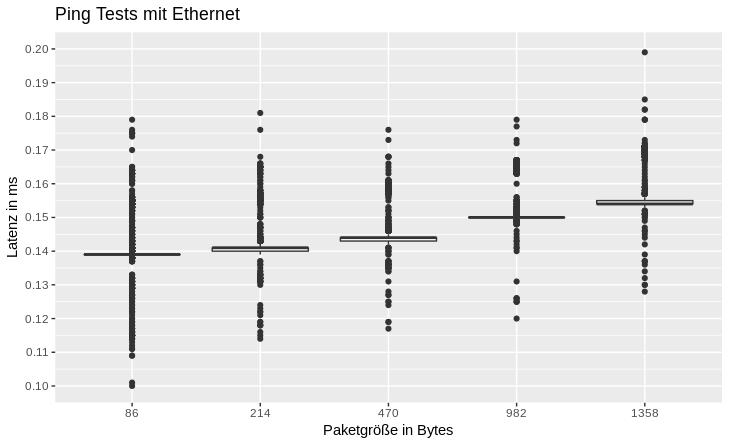
\includegraphics[width=1\textwidth]{images/Ethernetping.png}
\caption[Ping Diagramm mit Ethernet]{Das Boxplot Diagramm zeigt die Ping Tests mit normalen Ethernet Paketen. Es wurden 50.000 Tests durchgeführt. }
\label{img:CPU-WE8}
\end{figure}


\clearpage

%  Schlußfolgerungen, Fragen, Ausblicke

% Dieses Kapitel ist sicherlich das am Schwierigsten zu schreibende. Es
% dient einer gerafften Zusammenfassung dessen, was man gelernt hat. Es
% ist möglicherweise gespickt von Rückwärtsverweisen in den Text, um dem
% faulen aber interessierten Leser (der Regelfall) doch noch einmal die
% Chance zu geben, sich etwas fundierter weiterzubilden. Manche guten
% Arbeiten werfen mehr Probleme auf als sie lösen. Dies darf man ruhig
% zugeben und diskutieren. Man kann gegebenenfalls auch schreiben, was
% man in dieser Sache noch zu tun gedenkt oder den Nachfolgern ein paar
% Tips geben. Aber man sollte nicht um jeden Preis Fragen, die gar nicht
% da sind, mit Gewalt aufbringen und dem Leser suggerieren, wie
% weitsichtig man doch ist. Dieses Kapitel muß kurz sein, damit es
% gelesen wird.


%%% Local Variables:
%%% TeX-master: "diplom"
%%% End:


\appendix


%\addchap{Glossar}

%makeglossaries diplom


\deftranslation[to=German]{Acronyms}{Abkürzungsverzeichnis}
%\printglossary[style=altlist,title=Glossar]
\printglossary[type=\acronymtype,style=long]

%\printglossary[style=altlist]
%\printglossary[type=\acronymtype,style=long]

\printbibliography
\iffalse
    % an aid for Kile autocompletion
   % \bibliography{own.bib}
\fi

\end{document}
